%!TEX TS-program = xelatex
\documentclass[12pt, a4paper, oneside]{article}

% пакеты для математики 
\usepackage{amsmath,amsfonts,amssymb,amsthm,mathtools}  
\mathtoolsset{showonlyrefs=true}  % Показывать номера только у тех формул, на которые есть \eqref{} в тексте.

%Для подписи к матрицам
\usepackage{blkarray}

\usepackage[english, russian]{babel} % выбор языка для документа
% \usepackage[utf8]{inputenc}          % utf8 кодировка

% Основные шрифты 
\usepackage{fontspec}         
\setmainfont{Linux Libertine O}  % задаёт основной шрифт документа

% Математические шрифты 
\usepackage{unicode-math}     
\setmathfont[math-style=upright]{[Neo Euler.otf]} 


%%%%%%%%%% Работа с картинками и таблицами %%%%%%%%%%
\usepackage{graphicx} % Для вставки рисунков                
\usepackage{graphics}
\graphicspath{{images/}{pictures/}}   % папки с картинками

%С Геогебры для графика (by Yurec)
\usepackage{mathrsfs}
\usepackage{pgf,tikz,pgfplots}

\usepackage{wrapfig}    % обтекание рисунков и таблиц текстом

\usepackage{booktabs}   % таблицы как в годных книгах
\usepackage{tabularx}   % новые типы колонок
\usepackage{tabulary}   % и ещё новые типы колонок
\usepackage{float}      % возможность позиционировать объекты в нужном месте
\renewcommand{\arraystretch}{1.2}  % больше расстояние между строками

%by Dan4ik for geo5


%%%%%%%%%% Графики и рисование %%%%%%%%%%
\usepackage{tikz, pgfplots}  % языки для графики
\pgfplotsset{compat=1.16}
\usetikzlibrary{arrows}

\usepackage{todonotes} % для вставки в документ заметок о том, что осталось сделать
% \todo{Здесь надо коэффициенты исправить}
% \missingfigure{Здесь будет Последний день Помпеи}
% \listoftodos --- печатает все поставленные \todo'шки


%%%%%%%%%% Внешний вид страницы %%%%%%%%%%

\usepackage[paper=a4paper, top=20mm, bottom=15mm,left=20mm,right=15mm]{geometry}
\usepackage{indentfirst}    % установка отступа в первом абзаце главы

\usepackage{setspace}
\setstretch{1.15}  % межстрочный интервал
\setlength{\parskip}{4mm}   % Расстояние между абзацами
% Разные длины в LaTeX: https://en.wikibooks.org/wiki/LaTeX/Lengths

% свешиваем пунктуацию
% теперь знаки пунктуации могут вылезать за правую границу текста, при этом текст выглядит ровнее
\usepackage{microtype}

% \flushbottom                            % Эта команда заставляет LaTeX чуть растягивать строки, чтобы получить идеально прямоугольную страницу
\righthyphenmin=2                       % Разрешение переноса двух и более символов
\widowpenalty=300                     % Небольшое наказание за вдовствующую строку (одна строка абзаца на этой странице, остальное --- на следующей)
\clubpenalty=3000                     % Приличное наказание за сиротствующую строку (омерзительно висящая одинокая строка в начале страницы)
\tolerance=10000     % Ещё какое-то наказание.

% мои цвета https://www.artlebedev.ru/colors/
\definecolor{titleblue}{rgb}{0.2,0.4,0.6} 
\definecolor{blue}{rgb}{0.2,0.4,0.6} 
\definecolor{red}{rgb}{1,0,0.2} 
\definecolor{green}{rgb}{0,0.6,0} 
\definecolor{purp}{rgb}{0.4,0,0.8} 
\definecolor{dark_red}{rgb}{0.5,0,0} %by Yurec
\definecolor{qqqqtt}{rgb}{0.,0.,0.2}
\definecolor{cqcqcq}{rgb}{0.7529411764705882,0.7529411764705882,0.7529411764705882}


% цвета из geogebra 
\definecolor{litebrown}{rgb}{0.6,0.2,0}
\definecolor{darkbrown}{rgb}{0.75,0.75,0.75}
\definecolor{ududff}{rgb}{0.30196078431372547,0.30196078431372547,1.}
\definecolor{ffqqqq}{rgb}{1.,0.,0.}
\definecolor{xdxdff}{rgb}{0.49019607843137253,0.49019607843137253,1.}

% Гиперссылки
\usepackage{xcolor}   % разные цвета

\usepackage{hyperref}
\hypersetup{
	unicode=true,           % позволяет использовать юникодные символы
	colorlinks=true,       	% true - цветные ссылки
	urlcolor=blue,          % цвет ссылки на url
	linkcolor=black,          % внутренние ссылки
	citecolor=green,        % на библиографию
	breaklinks              % если ссылка не умещается в одну строку, разбивать её на две части?
}

%для сердечек(для души)
\usepackage{ marvosym }

% меняю оформление секций 
\usepackage{titlesec}
\usepackage{sectsty}

% выбрасываю нумерацию страниц и колонтитулы 
\pagestyle{empty}

% синие круглые бульпоинты в списках itemize 
\usepackage{enumitem}

\definecolor{itemizeblue}{rgb}{0, 0.45, 0.70}

\newcommand*{\MyPoint}{\tikz \draw [baseline, fill=itemizeblue, draw=blue] circle (2.5pt);}

\renewcommand{\labelitemi}{\MyPoint}

% расстояние в списках
\setlist[itemize]{parsep=0.4em,itemsep=0em,topsep=0ex}
\setlist[enumerate]{parsep=0.4em,itemsep=0em,topsep=0ex}

%%%%%%%%%% Свои команды %%%%%%%%%%

% Математические операторы первой необходимости:
\DeclareMathOperator{\sgn}{sign}
\DeclareMathOperator*{\argmin}{arg\,min}
\DeclareMathOperator*{\argmax}{arg\,max}
\DeclareMathOperator{\Cov}{Cov}
\DeclareMathOperator{\Var}{Var}
\DeclareMathOperator{\Corr}{Corr}
\DeclareMathOperator{\E}{\mathop{E}}
\DeclareMathOperator{\Med}{Med}
\DeclareMathOperator{\Mod}{Mod}
\DeclareMathOperator*{\plim}{plim}

% команды пореже
\newcommand{\const}{\mathrm{const}}  % const прямым начертанием
\newcommand{\iid}{\sim i.\,i.\,d.}  % ну вы поняли...
\newcommand{\fr}[2]{\ensuremath{^{#1}/_{#2}}}   % особая дробь
\newcommand{\ind}[1]{\mathbbm{1}_{\{#1\}}} % Индикатор события
\newcommand{\dx}[1]{\,\mathrm{d}#1} % для интеграла: маленький отступ и прямая d

% одеваем шапки на частые штуки
\def \hb{\hat{\beta}}
\def \hs{\hat{s}}
\def \hy{\hat{y}}
\def \hY{\hat{Y}}
\def \he{\hat{\varepsilon}}
\def \hVar{\widehat{\Var}}
\def \hCorr{\widehat{\Corr}}
\def \hCov{\widehat{\Cov}}

% Греческие буквы
\def \a{\alpha}
\def \b{\beta}
\def \t{\tau}
\def \dt{\delta}
\def \e{\varepsilon}
\def \ga{\gamma}
\def \kp{\varkappa}
\def \la{\lambda}
\def \sg{\sigma}
\def \tt{\theta}
\def \Dt{\Delta}
\def \La{\Lambda}
\def \Sg{\Sigma}
\def \Tt{\Theta}
\def \Om{\Omega}
\def \om{\omega}

% Готика
\def \mA{\mathcal{A}}
\def \mB{\mathcal{B}}
\def \mC{\mathcal{C}}
\def \mE{\mathcal{E}}
\def \mF{\mathcal{F}}
\def \mH{\mathcal{H}}
\def \mL{\mathcal{L}}
\def \mN{\mathcal{N}}
\def \mU{\mathcal{U}}
\def \mV{\mathcal{V}}
\def \mW{\mathcal{W}}

% Жирные буквы
\def \mbb{\mathbb}
\def \RR{\mbb R}
\def \NN{\mbb N}
\def \ZZ{\mbb Z}
\def \PP{\mbb{P}}
\def \QQ{\mbb Q}

%%%%%%%%%% Теоремы %%%%%%%%%%
\theoremstyle{plain} % Это стиль по умолчанию.  Есть другие стили.
\newtheorem{theorem}{Теорема}[section]
\newtheorem{result}{Следствие}[theorem]
% счётчик подчиняется теоремному, нумерация идёт по главам согласованно между собой

% убирает курсив и что-то еще наверное делает ;)
\theoremstyle{definition}         
\newtheorem*{definition}{Определение}  % нумерация не идёт вообще
\newtheorem*{remark}{Замечание}
  
% выделение по тексту важных вещей
\newcommand{\indef}[1]{\textbf{ \color{dark_red} #1}} 

\author{Ганыч Даниил \\ \href{https://vk.com/surealrzdnt}{surealrzdnt} \and Иванов Юрий \\ \href{https://vk.com/penzenskiy_ds}{penzenskiy\_ds} \and Никита Бекасов \\  \href{https://vk.com/k.onill}{k.onill}}



\title{Дискретная математика в \LaTeX}
\date{\today} 

\begin{document} % Конец преамбулы, начало файла

\maketitle

%\section*{Графы} 

%\begin{definition} 
%\indef{Граф} --- конечное множество вершин, а так же рёбер, соединяющих некоторые из этих вершин. Если важно, какая из вершин графа является первой, то такое ребро называется \indef{дугой} и обозначается вектором. Дуга присуща \indef{ориентированному графу.}
%\end{definition}

% Так можно делать пометки для себя, всё что за процентом не появится в pdf-ке

% Заметки, которые хочется чтобы появились
%\todo[inline]{Тут надо нарисовать картинку}

\section*{Предисловие}

Одной из фундаментальных наук, которые изучаются на нашем экономе, является дискретная математика. Именно этот предмет в будущем поможет Вам освоить более сложные и структурные дисциплины, или может стать неплохим стартом в изучении анализа данных. Данный проект задумывался как небольшая помощь будущим поколениям, ведь, несмотря на якобы «простоту» данного предмета (что на самом деле абсолютно не так), иногда очень трудно вникнуть в новую науку. 

Данная pdf-ка будет полезна тем, что здесь Вы найдете не только лекции Василия Павловича, размещенные в правильном хронологическом порядке, но и все заметки и примеры, которые он давал и которые помогли нам сдать экзамен и обязательно помогут Вам. Наличие этой pdf-ки не означает то, что Вы должны забить на посещение лекций Василия Павловича – наоборот, обязательно посещайте все его занятия, и сверяйте свои лекции с этими.


Отдельную благодарность мы хотим выразить Филиппу Ульянкину, ведь идейным вдохновителем данного проекта стал он и его старые лекции по дискретной математике, которыми мы пользовались во время подготовки к экзамену и которые затем решили реинкарнировать в электронном виде. Без тебя у нас бы ничего не получилось \Heart  


Также огромная благодарность выражается Решетникову Василию Павловичу, который является тем человеком, который не только знает свой предмет наизусть, но и способен передать свои знания другим поколениям. Вы, честно говоря, один из самых лучших и душевных преподавателей на экономическом факультете. Мы скучаем
\Heart \Heart \Heart 


Что же, предисловие подошло к своему логическому концу. Мы надеемся, что наш труд будет для Вас полезен. Занимайтесь математикой, развивайтесь и докажите, что вы – настоящие наследники эконома!



P.S: если у Вас будут предложения по корректировке материала, или, возможно, Василий Павлович даст более развернутые пояснения по некоторым темам, не стесняйтесь написать нам: \href{https://vk.com/penzenskiy_ds}{Юрий}, \href{https://vk.com/k.onill}{Никита},  \href{https://vk.com/surealrzdnt}{Даниил}. 


\hspace{1mm} \section*{Введение в дисциплину}

\begin{definition}
\indef{Дискретная математика} --- это раздел математики, в котором изучаются свойства конечных структур, а также бесконечных структур, в которых предполагается скачкообразность составляющих процессов или отделимость составляющих их элементов.
\end{definition}

В отличие от классической математики, здесь исследуется конечные структуры, 
а в классической - непрерывные. Деление математики на классическую и дискретную достаточно условное, т.к. наблюдается внедрения общих идей.

Бурное развитие дискретной математики вызвано развитием компьютерных технологий.
Современная дискретная математика включает в себя:
  
\begin{itemize}
    \item Теорию множеств;  
    \item Комбинаторику;        
    \item Теорию графов и сетей;
    \item Теорию кодирования;
    \item Теорию автоматов и т.д.
\end{itemize}

\section*{\textbf{Раздел I}}

\section*{Элементы теории множеств}

\section{Множество и операции над ними.}

\begin{definition}
Под \indef{множеством} понимается совокупность объектов любой природы, объединенных по какому либо признаку.\par
Объекты, составляющие множество, называются его \textit{элементами}.
Например: \par
\hspace{2mm} \textbf{A = \{a,b,c,d\}}, где \textbf{A} - произвольное множество, а \textbf{a,b,c,d} - его элементы.\par
Если каждый элемент множества \textbf{А} является элементом множества \textbf{B}, говорят, что множество \textbf{A} является \indef{подмножеством} множества \textbf{B}. 
\hspace{1cm} \[\textbf{A} \subseteq \textbf{B}\]

Если все элементы множества \textbf{A} являются подмножествами множества \textbf{B} и наоборот, это указывает на то, что \textbf{A} и \textbf{B} имеют одинаковые элементы и \textbf{A} = \textbf{B}.
\[ \textbf{A} = \textbf{B}\hspace{2mm} \Leftrightarrow \hspace{2mm} (\textbf{A} \subseteq \textbf{B}, \textbf{A} \supseteq \textbf{B}) \]

Множество, не содержащее ни одного элемента, - пустое множество. \varnothing \hspace{2mm} Считается, что пустое множество - подмножество любого множества. \par
Если число элементов конечное,то это конечное множество. Если число элементов множества бесконечное, то это бесконечное множество.
\end{definition}

 \indef{Множество можно задать:}
 \begin{enumerate}
    
     \item Перечислением его элементов, т.е. списком элементов: \[\textbf{A} = \{a,b,c,d\} \]
     
     \item Указанием характеристических свойств его элементов:
     \[\textbf{A} = \{x:P(x)\} \]
     
     \item Порождающей процедурой, т.е. множество задаётся совокупностью правил, по которым получаются элементы этого множества из уже известных элементов или других объектов. \par
     
     \underline{Пример}.
     
     \textbf{A} - множество целых чисел, являющихся степенями 2. Есть 2 правила:
     
     \begin{enumerate}
             \item 1 \in \hspace{1mm}\textbf{A};
     
             \item если \textbf{a} \in \hspace{1mm} \textbf{A}, то 
             
             \textbf{2a} \in \hspace{1mm} \textbf{A}.
     \end{enumerate}
     
     \end{enumerate} \par

Если \textbf{A} \(\subseteq\) \textbf{B} и \textbf{A} \neq \hspace{2mm} \textbf{B}, тогда множество \textbf{A} содержится во множестве \textbf{B}, или \textbf{B} содержит \textbf{A}. 
\par

Множества всех подмножеств множества \textbf{A} называется \indef{булеаном} этого множества. \par

\underline{Пример.}\hspace{2mm} \textbf{A} = \{1,2,3\} \Rightarrow
\(\varrho P\)(A) = \{\{1\},\{2\},\{3\},\{1,2\},\{1,3\},\{2,3\},\{1,2,3\},\{\varnothing\}\}. \par

\textbf{Число элементов} булеана - \(2^n\), где \(n\) - число элементов исходного множества. \par
Множество, которое содержит все множества при рассмотрении в данной задаче, называют универсальным. (\(U\)) \par 
\underline{Пример.} \\
\textbf{A} = \{1,2,3\} \\
\textbf{B} = \{2,4,9\} \\
\textbf{C} = \{2,3,5,10\} \\
\Rightarrow \(U\) = \{1,2,3,4,5,9,10\}. 

\section{Операции над множествами.}

  
  \begin{definition}
    
    \indef{Объединением} двух множеств \textbf{A} и \textbf{B} называют такое множество, которое состоит из тех и только тех элементов, которые принадлежат хотя бы одному множеству. 
    
    \[\textbf{A} \cup \textbf{B} = \{x: x \in \textbf{A} \hspace{1mm} \textrm{или} \hspace{1mm} x \in \textbf{B}\}\]
    
    Операции над множествами удобно изображать на диаграммах Эйлера-Венна: \par 

    Аналогично определяются объединения 3-х и более множеств.
    \end{definition}

    \begin{figure}[h!]
        
        \centering
        
        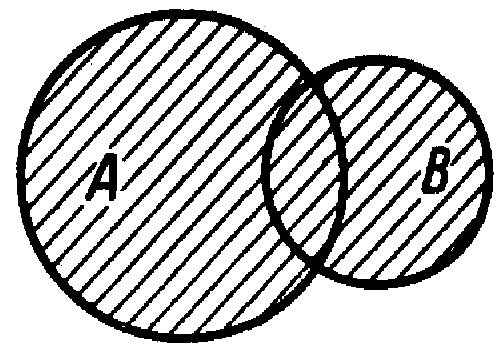
\includegraphics[width=0.3\textwidth]{reer.jpg}
       
    \end{figure}

  \begin{definition}
 
  \indef{Пересечением} множеств \textbf{A} и \textbf{B} называется такое множество, которое состоит из тех и только тех  элементов, которые принадлежат и \textbf{A}, и \textbf{B}.
  
  \[\textbf{A} \cap \textbf{B} = \{x: x \in \textbf{A} \hspace{1mm} 
  \textrm{и} \hspace{1mm} x\in \textbf{B}\}\]
  
   \end{definition}
  
  \begin{figure}[h!]
      
      \centering
      
      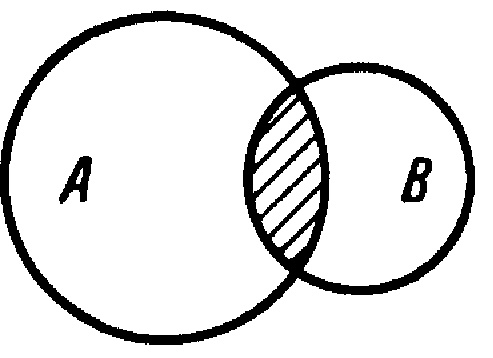
\includegraphics[width=0.3\textwidth]{erre.jpg}
      
  \end{figure}
  
  \begin{definition}
  
  \indef{Разностью} множеств \textbf{A} и \textbf{B} называется такое множество, которое состоит из тех и только тех элементов множества \textbf{A}, которые не содержатся в \textbf{B}.
  
  \[\textbf{A} \backslash \textbf{B} = \{x: x \in \textbf{A} \hspace{1mm} \textrm{и} \hspace{1mm} x \notin \textbf{B}\} \]
  
  \end{definition}

    \begin{figure}[h!]
       
        \centering
        
        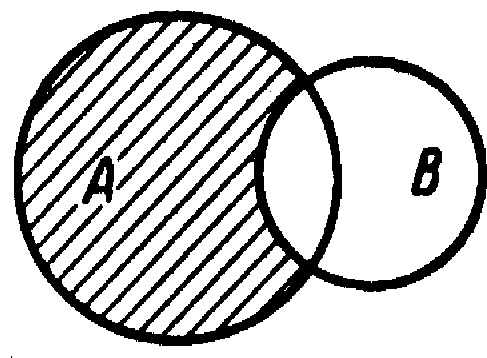
\includegraphics[width=0.3\textwidth]{yeezy.jpg}
        
    \end{figure}

\begin{definition}

\indef{Дополнением} множества \textbf{A} называют множества всех элементов универсального множества \(U\), не входящих во множество \textbf{A}.

\[\bar{A} = \{x: x \notin \mathbf{A} \hspace{1mm} \textrm{и} \hspace{1mm} x \in U \}\]

\end{definition}

\begin{figure}[h!]
    
    \centering
    
    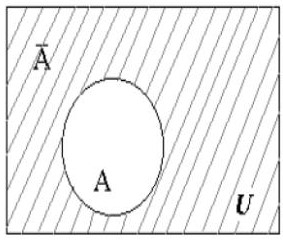
\includegraphics[width=0.25\textwidth]{kak.jpg}
    
\end{figure}

\begin{definition}

\indef{Симметрической разностью} (кольцевой суммой) называются множество, которое включает в себя все те элементы, которые принадлежат только одному из множеств.

\[\textbf{A} \oplus \textbf{B} = (\textbf{A} \backslash \textbf{B}) \cup (\textbf{B} \backslash \textbf{A})\]
\[\textbf{A} \oplus \textbf{B} =(\textbf{A} \cup \textbf{B}) \backslash (\textbf{B} \cup \textbf{A})\]

\end{definition}

\begin{figure}[h!]
    \centering
    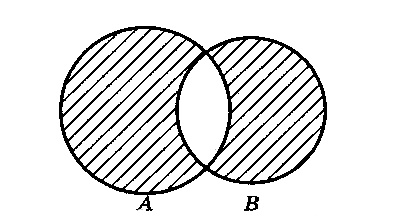
\includegraphics[width=0.45\textwidth]{ped.jpg}
\end{figure}

\section{Свойства операций над множествами(законы алгебры множеств).} 
\begin{enumerate}
    
    \item \textbf{Комутативный закон:}\\
    \(\textbf{A} \cup \textbf{B} = \textbf{B} \cup \textbf{A}\) \\
    \(\textbf{A} \cap \textbf{B} = \textbf{B} \cap \textbf{A}\)
    
    \item \textbf{Ассоциативный закон:}\\
    \(\textbf{A} \cup \textbf{B} \cup \textbf{C} = \textbf{A} \cup (\textbf{B} \cup \textbf{C})\) \\
     \(\textbf{A} \cap \textbf{B} \cap \textbf{C} = \textbf{A} \cap (\textbf{B} \cap \textbf{C})\)
     
     \item \textbf{Дистрибутивный закон:}\\
     \((\textbf{A} \cup \textbf{B}) \cap \textbf{C} = (\textbf{A} \cap \textbf{C}) \cup (\textbf{B} \cap \textbf{C})\) \\
     \((\textbf{A} \cap \textbf{B}) \cup \textbf{C} = (\textbf{A} \cup \textbf{C}) \cap (\textbf{B} \cup \textbf{C})\)
     
     \item \textbf{Законы двойственности(\emph{де Моргана}):}\\
     \(\bar{\bar{\textbf{A}} \cup \bar{\textbf{B}}} = \bar{\textbf{A}} \cap \bar{\textbf{B}} \) \\
     \(\bar{\bar{\textbf{A}} \cap \bar{\textbf{B}}} = \bar{\textbf{A}} \cup \bar{\textbf{B}} \)
    
     \item \textbf{Законы идемпотентности:} \\
     \(\textbf{A} \cup \textbf{A} = \textbf{A}\) \\
     \(\textbf{A} \cup \varnothing = \textbf{A}\) \\
     \(\textbf{A} \cup U = U\) \\
     \(\textbf{A} \cap \textbf{A} = \textbf{A}\) \\
     \(\textbf{A} \cap \varnothing = \varnothing\) \\
     \(\textbf{A} \cap U = \textbf{A}\)
    
     \item \textbf{Законы поглощения:} \\
     \(\textbf{A} \cup (\textbf{A} \cap \textbf{B}) = \textbf{A}\) \\
     \(\textbf{A} \cap (\textbf{A} \cup \textbf{B}) = \textbf{A}\)
    
     \item \textbf{Законы включения:}
     \(\textbf{A} \subseteq \textbf{B} \Leftrightarrow \bar{\textbf{B}} \subseteq \bar{\textbf{A}} \)
    
     \item \textbf{Законы двойного дополнения:} \\
     \(\bar{\bar{\textbf{A}}} = \textbf{A}\)
    
     \item \textbf{Законы равенства:} \\
     \(\textbf{A} = \textbf{B} \Leftrightarrow (\textbf{A} \subseteq \textbf{B}) \cap (\textbf{B} \subseteq \textbf{A})\)
\end{enumerate}

\section{Декартово произведение множеств.}

Пусть даны \textbf{A} и \textbf{B}, пара (a, b), где a \in \hspace{2mm} \textbf{A}, b \in \hspace{2mm} \textbf{B}. Такая пара называется \emph{упорядоченной}, причём (a, b) и (\(a_1\), \(b_1\)) считаются одинаковыми, если a = \(a_1\), b = \(b_1\). 

\begin{definition}

Множество всех упорядоченных пар вида (a, b), где a \in \textbf{A}, b \in \textbf{B}, называется \indef{декартовым(или прямым) произведением} множеств \textbf{A} и \textbf{B}:

\[\textbf{A} \times \textbf{B} = \{\textbf{(a,b)}: \textbf{a} \in \textbf{A}, \textbf{b} \in \textbf{B}\}\]

\[\textbf{A} \times \textbf{B} \neq \textbf{B} \times \textbf{A}\]

\end{definition}

\begin{definition}

Пусть даны множества \textbf{\(A_1\)}, \textbf{\(A_2\)}, \textbf{\(A_3\)}, ... Декартовым произведением этих множеств называется множества упорядоченных наборов $a_1$, \(a_2\), \(a_3\), ... , где \(a_1\) \in \(A_1\), \(a_2\) \in \(A_2\), \(a_3\) \in \(A_3\), ..., \(a_n\) \in \(A_n\):

\[
A_1 \times A_2 \times ... \times A_n = \{(a_1, a_2, ... , a_n): a_1 \in A_1, a_2 \in A_2, ... , a_n \in A_n\}
\]

В частности, если \(A_1\) = \(A_2\) = ... = \(A_n\), то \hspace{1mm} \(A_1 \times A_2 \times ... \times A_n = A^n\) --- \emph{декартова степень}.
\end{definition}

Отметим некоторые \textbf{свойства} декартова произведения:

\begin{enumerate}
    
    \item \((\textbf{A} \cup \textbf{B}) \times \textbf{C} = (\textbf{A} \times \textbf{C}) \cup (\textbf{B} \times \textbf{C})\)
    
    \item \((\textbf{A} \cap \textbf{B}) \times \textbf{C} = (\textbf{A} \times \textbf{C}) \cap (\textbf{B} \times \textbf{C})\)
    
    \item \((\textbf{A} \backslash \textbf{B}) \times \textbf{C} = (\textbf{A} \times \textbf{C}) \backslash (\textbf{B} \times \textbf{C})\)
    
    \item \(\textbf{C} \times  (\textbf{A} \backslash \textbf{B}) = (\textbf{C} \times \textbf{A}) \backslash (\textbf{C} \times \textbf{B})\)
    
\end{enumerate}


\(\blacksquare\) \textbf{Доказательство свойства 2}:
\begin{enumerate}
    
\item \((x, y) \in (A \cap B) \times C \Longrightarrow x \in (A \cap B) \wedge y \in C \Longrightarrow x \in A \wedge x \in B \wedge y \in C \Longrightarrow (x, y) \in (A \times C) \wedge (x, y) \in (B \times C) \Longrightarrow (x, y) \in (A \times C) \cap (B \times C).\) 


\((A  \cap B) \times C  \subseteq (A \times C) \cap (B \times C) \ast\) 

\item \((x, y) \in (A \times C) \cap (B \times C) \Longrightarrow (x, y) \in (A \times C) \wedge (x, y) \in (B \times C) \Longrightarrow x \in A \wedge y \in C \wedge x \in B \wedge y \in C \Longrightarrow x \in (A \cap B) \wedge y \in C \Longrightarrow (x, y) \in (A  \cap B) \times C.\) 


\((A \times C) \cap (B \times C) \subseteq (A  \cap B) \times C  \ast \ast \) 

\end{enumerate}

На основании включений \(\ast\)  и \(\ast \ast\)  делаем вывод, что свойство 2 - доказано. 

\section{Мощность декартова произведения множеств.}

Пусть \textbf{A} и \textbf{B} - конечные множества.

\begin{definition}
\indef{Мощностью} \emph{конечного} множества называется число элементов этого множества. 
\end{definition}

\begin{theorem}
Мощность декартова произведения конечного числа конечных множеств равно произведению мощностей этих множеств:

\[|A_1 \times A_2 \times ... \times  A_n| = |A_1| \times |A_2| \times ... \times |A_n|\], где |...| - мощность множества.
\end{theorem}

\(\blacksquare\)\textbf{Доказательство (методом математической индукции):}


\underline{Суть метода:} проверяется справедливость доказуемого  утверждения при n = 1. Далее, мы предполагаем, что доказанное утверждение справедливо при n = k. И нам остаётся доказать, что утверждение справедливо при n = k + 1. 


При n = 1: 


\(|A_1| = m_1\) - верно. 


Предположим, что \(|A_1 \times A_2 \times ... \times A_k| = m_1 \cdot m_2 \cdot... \cdot m_k\) - верно. 


Проверим для n = k + 1. Возьмём \(|A_1 \times A_2 \times ... \times A_k|\), тогда для этого декартова произведения \(m_1 \cdot m_2 \cdot ... \cdot m_K\) наборов решений \((a_1, a_2, ... , a_k)\), где $a_1 \in A_1$, $a_2 \in A_2$, $a_k \in A_k$. 


$a_k+1 \in A_k+1$ $\Longrightarrow$ \((a_1, a_2, ... , a_k, a_k+1) \in |A_1 \times A_2 \times ... \times A_k \times A_k+1|\). 


Так как мощность $|A_1 \times A_2 \times ... \times A_k = m_1 \cdot m_2 \cdot... \cdot m_K$, то из этого следует, что число элементов 
$A_1 \times A_2 \times ... \times A_k \times A_k+1$ равна $m_1 \cdot m_2 \cdot... \cdot m_k \cdot m_k+1$. То есть:


$|A_1 \times A_2 \times ... \times A_k \times A_k+1| = m_1 \cdot m_2 \cdot... \cdot m_k \cdot m_k+1 $ 

 
Следовательно доказываемое утверждение справедливо.

\section*{Отношения и функции}

Для характеристики взаимосвязей между элементами одного или нескольких множеств вводится понятие отношения множества. Наиболее часто встречаются одноместные (унарные) отношения и двухместные (бинарные) отношения. \par

Пусть дано множество \textbf{A}, тогда его элементы, обладающие некоторыми свойствами составляют некоторые подмножества множества \textbf{A}. Это подмножество называют одноместным (или унарным) отношением множества \textbf{A} и состоит из элементов с определёнными свойствами. Таким образом одноместное отношение на множестве характеризуют какое-то свойство элементов этого множества. $P \subseteq A$.\par

Бинарное отношение характеризует взаимосвязь между элементами одного или двух множеств, и их часто называют соответствием. Бинарное отношение представляет собой подмножество декартова произведения $A \times B$ или $A \times A = A^2$. 

\[P \subseteq A \times B \hspace{3cm} P = \{(a,b): a \in A, b \in B\}\]
\[P \subseteq A^2 \hspace{3.53cm} P = \{(a,b): a \in A, b \in A\}\] \par

В общем случае можно определить n-местное отношение между элементами множеств $A_1, A_2, ... , A_n$.

\section{Бинарное отношение. Основные понятия.}

Пусть даны множества \textbf{A} и \textbf{B}.

\begin{definition}
\indef{Бинарным отношением} на этих множествах называется подмножество декартова произведения $\textbf{A} \times \textbf{B}$: $\textbf{P} \subseteq \textbf{A} \times \textbf{B}$.
\end{definition}

В частности, если \textbf{A} = \textbf{B}, то $\textbf{P} \subseteq \textbf{A}^2$ \par

\underline{Пример.} \\ Пусть \textbf{A} = \textbf{B} = \{2,3,4,5,6,7,8\}, \hspace{2mm}
$\textbf{P} \subseteq \textbf{A} \times \textbf{B} = \textbf{A}^2$. 


\textbf{P} = \{(a,b): a \in \textbf{A}, b \in \textbf{B}, b делится на a нацело, причем a \leq \hspace{2mm} 4\} 


Зададим это бинарное отношение списком:


\textbf{P} = \{(2,2),(2,4),(2,6),(2,8),(3,3),(3,6),(4,4),(4,8)\}.

\begin{definition}
\indef{Областью определения} $D_p$ бинарного отношения $\textbf{P} \subseteq \textbf{A} \times \textbf{B}$ называется $D_p = \{a: a \in A, причём (a,b) \in \textbf{P}, b \in \textbf{B}\}$. 
\end{definition}

\begin{definition}
\indef{Множеством значений} $R_p$ бинарного отношения $\textbf{P} \subseteq \textbf{A} \times \textbf{B}$ называется множество $R_p = \{b: b \in \textbf{B}, (a,b) \in \textbf{P},
a \in \textbf{A}\}$.
\end{definition}

Итак, в приведенном выше примере: 
$D_p = \{2,3,4\}$ \\
$R_p = \{2,3,4,6,8\}$

\begin{definition}
\indef{Образом элемента} $a \in \textbf{A}$ при бинарном отношении $\textbf{P} \subseteq \textbf{A} \times \textbf{B}$ называется множество $P(a) = \{b: b \in \textbf{B}, (a,b) \in \textbf{P}\}$.
\end{definition}

Так, в приведенном выше бинарном отношении: 


$P(2) = \{2,4,6,8\}$

\begin{definition}
\indef{Прообразом элемента} $b \in \textbf{B}$ при $\textbf{P} \subseteq \textbf{A} \times \textbf{B}$ называется множество $P^{-1} (b) = \{a: a \in \textbf{A}, (a,b) \in \textbf{P}\}$.
\end{definition}

Так, в рассматриваемом бинарном отношении: 


\(P^{-1}(6) = \{2,3\}\)

\begin{definition}
Пусть $\textbf{P} \subseteq \textbf{A} \times \textbf{B}$ и \textbf{C} \subseteq \textbf{A}. \indef{Образом} подмножества \textbf{C} называется объединение образов всех элементов подмножества \textbf{C}: $P(\textbf{C}) = \cup P(a), a \in \hspace{1mm}\textbf{C}$
\end{definition}

Так в рассматриваемом примере: 


C =\{3,4\}, то $P(C) = P(3) \cup P(4) = \{3,6\} \cup \{4,8\} = \{3,4,6,8\}$.

\begin{definition}
\indef{Прообразом} подмножества $\textbf{D} \in \textbf{B}$ при $\textbf{P} \subseteq \textbf{A} \times \textbf{B}$ называется объединение всех прообразов подмножества \textbf{D}: $P^{-1}(\textbf{D}) = \cup P^{-1}(b), b \in \textbf{D}$.
\end{definition}

\begin{definition}
Пусть $\textbf{P} \subseteq \textbf{A} \times \textbf{B}$, \indef{обратным отношением} $P^{-1}$ называется множество $P^{-1} = \{(b,a): (a,b) \in \textbf{P}\}$.
\end{definition}

\begin{definition}
Пусть бинарное отношение $\textbf{P} \subseteq \textbf{A} \times \textbf{A}$ и $\textbf{P} = \{(x,x): x \in \textbf{A}\}$. Это бинарное отношение называется \indef{тождественным}.

Бинарное отношение можно изобразить графически. Это можно сделать разными способами. Например, пусть надо бинарное отношение $\textbf{P} = \{(x,y): x \in \textbf{A}, y \in \textbf{B}\}$, $\textbf{P} \subseteq \textbf{A} \times \textbf{B}$.


   Элементы множества \textbf{A} расположим на оси абсцисс, элементы множества \textbf{B} на оси ординат. Паре (x,y) соответствует точка на плоскости. 
   
   
   \textbf{A} = \{1,2,3\}, \textbf{B} = \{1,2,3,4\}
   
   
   \textbf{P} = \{(1,1),(1,3),(2,2),(3,1),(3,4)\}
   \end{definition}
   
\begin{figure}[H]
\centering
\begin{tikzpicture}[line cap=round,line join=round,>=triangle 45,x=1.0cm,y=1.0cm]
\begin{axis}[
x=1.0cm,y=1.0cm,
axis lines=middle,
ymajorgrids=true,
xmajorgrids=true,
xmin=-0.3,
xmax=4.0,
ymin=-0.3,
ymax=4.5,
xtick={-0.0,1.0,...,4.0},
ytick={-0.0,1.0,...,4.0},]
\clip(-0.3,-0.3) rectangle (4.,4.5);
\begin{scriptsize}
\draw [fill=ududff] (1.,1.) circle (2.5pt);
\draw[color=ududff] (1.0836115546400176,1.2086130641977466) node {$A$};
\draw [fill=ududff] (1.,3.) circle (2.5pt);
\draw[color=ududff] (1.0836115546400176,3.2097640989536287) node {$B$};
\draw [fill=ududff] (2.,2.) circle (2.5pt);
\draw[color=ududff] (2.084187072017961,2.2091885815756878) node {$C$};
\draw [fill=ududff] (3.,1.) circle (2.5pt);
\draw[color=ududff] (3.084762589395904,1.2086130641977466) node {$D$};
\draw [fill=ududff] (3.,4.) circle (2.5pt);
\draw[color=ududff] (3.084762589395904,4.210339616331569) node {$E$};
\end{scriptsize}
\end{axis}
\end{tikzpicture}
\end{figure} 
   
Другой возможный вариант графического изображения:

\begin{figure}[h!]
 \centering
  \begin{tikzpicture}[line cap=round,line join=round,>=triangle 45,x=1.0cm,y=1.0cm]
\clip(-2.,-1.5) rectangle (6.,2.6);
\draw [rotate around={-87.66269414087635:(-0.3083035332010371,0.5233638937501102)},line width=2.pt] (-0.3083035332010371,0.5233638937501102) ellipse (1.7687684594597688cm and 1.4913791043789708cm);
\draw [rotate around={-88.92917554520933:(4.500728443867752,0.6881895865125487)},line width=2.pt] (4.500728443867752,0.6881895865125487) ellipse (1.7518856234265408cm and 1.4115457613826754cm);
\draw [->,line width=0.5pt] (-0.3470860491451403,1.4735355343806376) -- (4.4813371858957005,1.725621888017308);
\draw [->,line width=0.5pt] (-0.3470860491451403,1.4735355343806376) -- (4.520119701839803,-0.3492427149922106);
\draw [->,line width=0.5pt] (-0.269521017256934,-0.42680774688041695) -- (4.520119701839803,0.5427551517221618);
\draw [->,line width=0.5pt] (-0.32769479117308875,0.5621464096942135) -- (4.500728443867752,1.1826666647998638);
\draw [->,line width=0.5pt] (-0.32769479117308875,0.5621464096942135) -- (4.520119701839803,0.5427551517221619);
\draw [->,line width=0.5pt] (-0.269521017256934,-0.42680774688041695) -- (4.520119701839803,-0.34924271499221066);
\begin{scriptsize}
\draw [fill=ududff] (-0.3470860491451403,1.4735355343806376) circle (2.5pt);
\draw[color=ududff] (-0.2113472433407793,1.8322738068635918) node {$A$};
\draw [fill=ududff] (-0.269521017256934,-0.42680774688041695) circle (2.5pt);
\draw[color=ududff] (-0.13378221145257302,-0.06806947439746278) node {$B$};
\draw [fill=ududff] (-0.32769479117308875,0.5621464096942135) circle (2.5pt);
\draw[color=ududff] (-0.19195598536872777,0.9208846821771677) node {$C$};
\draw [fill=ududff] (4.4813371858957005,1.725621888017308) circle (2.5pt);
\draw[color=ududff] (4.617075991700061,2.084360160500262) node {$D$};
\draw [fill=ududff] (4.520119701839803,-0.34924271499221066) circle (2.5pt);
\draw[color=ududff] (4.655858507644164,0.009495557490743545) node {$E$};
\draw [fill=ududff] (4.500728443867752,1.1826666647998638) circle (2.5pt);
\draw[color=ududff] (4.636467249672113,1.541404937282818) node {$G$};
\draw [fill=ududff] (4.520119701839803,0.5427551517221619) circle (2.5pt);
\draw[color=ududff] (4.655858507644164,0.901493424205116) node {$H$};
\end{scriptsize}
\end{tikzpicture}
\end{figure}

Бинарное отношение $\textbf{P} \subseteq A^2$, \textbf{A} = \{a,b,c,d\}, \textbf{P} = \{(a,a),(a,b),(b,b),(b,d),(c,c),(c,d)\} можно изобразить следующим образом:

\begin{figure}[h!] %оказывается, тех падает от freehand, пришлось картинку пихать ((( 
\centering
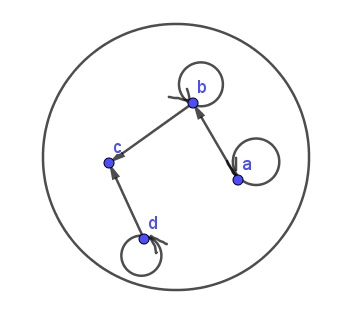
\includegraphics[width=0.4\textwidth]{dfgh.jpg}
\end{figure}

\section{Операции над бинарными отношениями.}
Так как бинарное отношение - это подмножество декартова произведения двух множеств, то над бинарными отношениями можно выполнить те же операции, что и над множествами.\par

Пусть $\textbf{P}_1 \subseteq \textbf{A} \times \textbf{B}$, $\textbf{P}_2 \subseteq \textbf{A} \times \textbf{B}$.
\begin{enumerate}
    
    \item $\textbf{P}_1 \cup \textbf{P}_2$ = $\{(a,b) : (a,b) \in \textbf{P}_1 \vee (a,b) \in \textbf{P}_2\}$
    
    \item $\textbf{P}_1 \cap \textbf{P}_2$ = $\{(a,b) : (a,b) \in \textbf{P}_1 \wedge (a,b) \in \textbf{P}_2\}$
    
    \item $\textbf{P}_1 \backslash \textbf{P}_2$ = $\{(a,b) : (a,b) \in \textbf{P}_1 \wedge (a,b) \notin \textbf{P}_2\}$
    
    \item $\bar{P}_1$ = $(\textbf{A} \times \textbf{B}) \backslash \textbf{P}_2$ \\
    $\bar{P}_1$ = $\{(a,b): (a,b) \in (\textbf{A} \times \textbf{B}) \wedge (a,b) \notin \textbf{P}_1\}$
    
    \item $\textbf{P}_1 \oplus \textbf{P}_2$ = $(\textbf{P}_1 \backslash \textbf{P}_2) \cup (\textbf{P}_2 \backslash \textbf{P}_1)$
    
    \item Композиция или произведение бинарных отношений. \\
    Пусть $\textbf{P}_1 \subseteq \textbf{A} \times \textbf{B}$, $\textbf{P}_2 \subseteq \times \textbf{B} \times \textbf{C}$.
    \begin{definition}
    
    Композицией(или произведением) этих бинарных отношений называется бинарное отношение $\textbf{P}_1 \circ \textbf{P}_2$, определяемое следующим образом:
    
    
    $\textbf{P}_1 \circ \textbf{P}_2 = \{(a,b): a \in \textbf{A}, b \in \textbf{C}, \exists x \in \textbf{B}: (a,x) \in \textbf{P}_1, (x,b) \in \textbf{P}_2\}$
    \end{definition}
    
\end{enumerate}

\underline{Пример.} Пусть $\textbf{P}_1 \subseteq \mathbb{N}^2$, где $\mathbb{N}^2$ - множество натуральных чисел, $\textbf{P}_1 = \{(a,b): a \in \mathbb{N}, b \in \mathbb{N}, b = 2a\}$ 


$\textbf{P}_2 \subseteq \mathbb{N}^2$,  $\textbf{P}_2 = \{(a,b): a \in \mathbb{N}, b \in \mathbb{N}, b = a^2 + 5\}$


$\textbf{P}_1 \circ \textbf{P}_2 = \{(a,b): a \in \mathbb{N}, b \in \mathbb{N}, \exists x \in \mathbb{N}: (a,x) \in \textbf{P}_1, (x,b) \in \textbf{P}_2\}$ = $\{(a,b): a \in \mathbb{N}, b \in \mathbb{N},  x \in \mathbb{N}: x = 2a, b = x^2 + 5\}$ = $\{(a,b): a \in \mathbb{N}, b \in \mathbb{N}, b = 4a^2 + 5\}$. 


$\textbf{P}_1 \circ \textbf{P}_2$ = $\{(a,b): a \in \mathbb{N}, b \in \mathbb{N}, b = 4a^2 + 5\}$. \par 

$\square$ \emph{Замечание.} Пусть $\textbf{P} \subseteq \textbf{A} \times \textbf{B}$ и $\textbf{Q} \subseteq \textbf{A} \times \textbf{B}$ - два бинарных отношения, и $\textbf{Q} \subseteq \textbf{P}$, то часто бинарное отношение \textbf{Q} называют \indef{сужением} бинарного отношения \textbf{P}.

\section{Матрица бинарного отношения.}
Бинарное отношение на конечных множествах часто задают с помощью матрицы.\par 

Пусть \textbf{A} = $\{a_1, a_2, a_3, ..., a_n\}$, \textbf{B} = $\{b_1, b_2, b_3, ..., b_m\}$, $\textbf{P} \subseteq \textbf{A} \times \textbf{B}$ - бинарное отношение. 
\begin{definition}

Матрицей бинарного отношения $\textbf{P} \subseteq \textbf{A} \times \textbf{B}$ называется матрица размерности $n \times m$, элементы которой определяются следующим образом:



$$ 
\mathbf{P}_{ij} =
\begin{cases}
1, \textrm{eсли} (a_i, b_j) \in \mathbf{P} \\
0, \textrm{если} (a_i, b_j) \notin \mathbf{P}
\end{cases}
$$
%\begin{cases}
%\textbf{P}_{ij} = 1, \textrm{eсли} (a_i, b_j) \in \textbf{P} \\
%0, \textrm{если} (a_i, b_j) \notin \textbf{P}
%\end{cases}

\end{definition}

\underline{Пример.}\par

\textbf{A} = \{1,2,3\}, \hspace{2mm} \textbf{P} = \{(1,1),(1,2),(2,2),(3,3)\}. Запишем матрицу \textbf{[P]}: \[\textbf{[P]} =
\begin{pmatrix}
1 & 1 & 0\\
0 & 1 & 0\\
0 & 0 & 1
\end{pmatrix}\]

Очевидно, что любая матрица, состоящая из 0 и 1 может рассматриваться как матрица бинарного отношения. \par 

Пусть даны $\textbf{P} \subseteq \textbf{A} \times \textbf{B}$, $\textbf{Q} \subseteq \textbf{A} \times \textbf{B}$. Отметим следующие \indef{свойства} матриц бинарного бинарного отношения:

\begin{enumerate}
    
    \item Матрица a равна сумме матриц этих отношений: $[\textbf{P} \cup \textbf{Q}] = [\textbf{P}] + [\textbf{Q}]$, причем сложение элементов матриц равно: 0 + 0 = 0, 1 + 0 = 0, 1 + 1 = 1.
    
    \item Матрица $\textbf{P} \cap \textbf{Q}$ пересечения этих бинарных отношений равна: $[\textbf{P} \cap \textbf{Q}] = [\textbf{P}] * [\textbf{Q}]$, где $*$ - поэлементное умножение.
    
    
    \underline{Пример.} [\textbf{P}] = $\begin{psmallmatrix}
    1 & 0 & 1 & 1\\
    0 & 1 & 0 & 1
    \end{psmallmatrix}$, [\textbf{Q}] = $\begin{psmallmatrix}
    0 & 0 & 0 & 1\\ 
    1 & 1 & 1 & 0
    \end{psmallmatrix}$. Тогда: $[\textbf{P} \cap \textbf{Q}] = [\textbf{P}] * [\textbf{Q}] = \begin{psmallmatrix}
    1 & 0 & 1 & 1\\
    0 & 1 & 0 & 1
    \end{psmallmatrix} * \begin{psmallmatrix}
    0 & 0 & 0 & 1\\ 
    1 & 1 & 1 & 0
    \end{psmallmatrix} = \begin{psmallmatrix}
    0 & 0 & 0 & 1\\
    0 & 1 & 0 & 0
    \end{psmallmatrix}$  
    
    \item Пусть $\textbf{P} \subseteq \textbf{A} \times \textbf{B}$, $\textbf{Q} \subseteq \textbf{B} \times \textbf{C}$ - два бинарных отношения. Тогда $[\textbf{P} \circ \textbf{Q} = [\textbf{P}] \cdot [\textbf{Q}]$, причем матрицы перемножаются по правилам линейной алгебры, а сумма элементов:\\ 0 + 0 = 0, 0 + 1 = 1, 1 + 1 = 1.
    
    \item Матрица отношения $\textbf{P}^{-1}$ обратного для отношения \textbf{P} равна транспонированной матрице отношения \textbf{P}: $[\textbf{P}^{-1}] = [\textbf{P}^T]$. 
    
    \item Матрица тождественного отношения - это единичная матрица.
    
    \item Если $\textbf{P} \subseteq \textbf{A} \times \textbf{B}$, $\textbf{Q} \subseteq \textbf{A} \times \textbf{B}$ и $\textbf{Q} \subseteq \textbf{P}$ \hspace{2mm}(т.е.сужение \textbf{P}) \Rightarrow $q_{ij} \subseteq p_{ij}$.
\end{enumerate}

\section{Свойства бинарных отношений.}

Рассмотрим бинарные отношения, заданные на непустом множестве \textbf{A}.

\begin{definition}
Бинарное отношение $\textbf{P} \subseteq \textbf{A} \times \textbf{A}$ называется \indef{рефлексивным}, если для всех $x$ из \textbf{A} выполняется $(x,x) \in \textbf{P}$. Если множество \textbf{A} - конечное множество и бинарное отношение $\textbf{P} \subseteq \textbf{A} \times \textbf{A}$ - рефлексивное, то главная диагональ матрицы рефлексивного на этом множестве отношения содержит только единицы. 
\end{definition}

\begin{definition}
Бинарное отношение $\textbf{P} \subseteq \textbf{A} \times \textbf{A}$ называется \indef{антирефлексивным}, если для всех $x \in \textbf{A}$ выполняется $(x,x) \notin \textbf{p}$. Если множество \textbf{A} - конечное множество и бинарное отношение $\textbf{P} \subseteq \textbf{A} \times \textbf{A}$ - антирефлексивное,то главная диагональ матрицы такого отношения состоит из нулей. 
\end{definition}


\underline{Пример 1.}
\begin{enumerate}

\item $\textbf{P} \subseteq R$, $\textbf{P} = \{(x,y): x \in R, y \in R, x \leq y\}$ - это отношение будет рефлексивным, т.к. $x \in R, (x,x) \in \textbf{P} \Rightarrow x \leq x$. 


\item $\textbf{P} \subseteq R$, $\textbf{P} = \{(x,y): x \in R, y \in R, x < y$ - это отношение будет антирефлексивным, т.к. $x \in \textbf{A}, (x,x) \notin \textbf{P} \Leftrightarrow x < x$.

\end{enumerate}

\begin{definition}
Бинарное отношение $\textbf{P} \subseteq \textbf{A} \times \textbf{A}$ называется \indef{симметричным}, если из $(x,y) \in \textbf{P} \Rightarrow (y,x) \in \textbf{P}$. Если множество \textbf{A} -  конечное, то матрица симметричного бинарного отношения на этом множестве симметрична относительно главной диагонали.
\end{definition}


\underline{Пример 2.}


\textbf{A} = \{1,2,3,4,5,6\}, $\textbf{P}\subseteq\textbf{A}\times\textbf{A}$, \textbf{P} = \{(x,y): x \in \textbf{A}, y \in \textbf{A}, \textrm{x и y имеют общий делитель, отличный от единицы}\} - такое отношение симметрично. 

\begin{definition}
Бинарное отношение $\textbf{P} \subseteq \textbf{A} \times \textbf{A}$ называется \indef{антисимметричным}, если $(x,y) \in \textbf{P}$ и $(y,x) \in \textbf{P} \Rightarrow x = y$. 
\end{definition}


Рассмотренный выше пример 1 является примером антисимметричного отношения. Пусть $(x,y) \in \textbf{P}$ и $(y,x) \in \textbf{P} \Rightarrow ? x = y$ 


$(x,y) \in \textbf{P}$ \Rightarrow $x \leq y$ $(y,x) \in \textbf{P}$


\Rightarrow $y \leq x$ \Rightarrow $x = y$. \par


Отметим, что несимметричность отношения не означает, что это отношение будет антисимметрично. 


\textbf{A} = \{1,2,3\}, $\textbf{P} = \{(1,2), (2,3), (3,2)\}$ 


$(1,2) \in \textbf{P}$ и $(2,1) \notin \textbf{P}$ \Rightarrow отношение несимметрично. 


$(2,3) \in \textbf{P}$ и $(3,2) \in \textbf{P}$, но $2 \neq 3 \Rightarrow$ отношение не является антисимметричным.\par 

Для того, чтобы по матрице бинарного отношения определить, будет ли оно антисимметрично, нужно: $[\textbf{P}]*[\textbf{P}]^T$($*$ умножение соответствующих элементов). Если у полученной матрицы все элементы, стоящие вне главой диагонали - нулевые, то эта матрица - антисимметрична. 

\begin{definition}
Бинарное отношение $\textbf{P} \subseteq \textbf{A} \times \textbf{A}$ называется транзитивным, если из $(x,y) \in \textbf{P}$ и $(y,z) \in \textbf{P} \Rightarrow (x,z) \in \textbf{P}$.
\end{definition}

\underline{Пример.}


Пусть $\textbf{P} \subseteq R^2, \textbf{P} = \{(x,y):x \in R, y \in R, x \leq y\}$


Из $(x,y) \in \textbf{P} \Rightarrow x \leq y$ и $(y,z) \in \textbf{P} \Rightarrow y \leq z$. Будет ли $\Rightarrow? x \leq z$. Проверим: т.к. $x \leq y$ и $y \leq z$, то $x \leq z, \Rightarrow$ это отношение транзитивно.\par


Если множество \textbf{A} - конечное и на нём задано бинарное отношение $\textbf{P} \subseteq \textbf{A} \times \textbf{A}$, то с помощью матрицы этого отношения можно проверить, будет ли это отношение транзитивно. Для этого нужно умножить матрицу на себя по правилам линейной алгебры(сложение по правилу 0 + 0 = 0, 0 + 1 = 1, 1 + 1 = 1), и если в результате получится исходная матрица, то отношение транзитивно: $[\textbf{P}][\textbf{P}] = [\textbf{P}]$

\section{Отношение эквивалентности.}

\begin{definition}
Бинарное отношение на множестве \textbf{A} $\textbf{P} \subseteq \textbf{A} \times \textbf{A}$ называется отношением эквивалентности(или просто эквивалентностью), если оно рефлексивно, симметрично и транзитивно. $E \subseteq \textbf{A} \times \textbf{A}$. Другие возможные обозначения: $xEy$, $(x,y) \in E$, $x \sim y$.
\end{definition}

\begin{definition}
Классом эквивалентности элемента $x \in \textbf{A}$ называется множество $E(x) = \{y: y \in \textbf{A}, (x,y) \in E\}$.
\end{definition}

\begin{definition}
Множество классов эквивалентности элементов $x \in \textbf{A}$ по отношению к эквивалентности $E$ называется фактором множества \textbf{A} по отношению к $E$. $A/E = \{E(x), x \in \textbf{A}\}$. 
\end{definition}

\begin{definition}
Совокупность множеств $\{A_i\}$ называется разбиением множества \textbf{A}, если $A_i$ - непустые, $A_i \cap A_j = \varnothing$ при $i \neq j$, $\bigcup_{i}A_i = A$.
\end{definition}

\begin{theorem}

\begin{enumerate}
    
    \item Фактор множества $A/E = \{E(x), x \in \textbf{A}\}$ является разбиением множества \textbf{A}.
    
    \item Если $\{A_i\}$ - это разбиение множества \textbf{A}, то на множестве \textbf{A} можно задать соответствующее этому разбиению отношение эквивалентности $\mathbb{A} \Rightarrow E$.

\end{enumerate}

\end{theorem}

$\blacksquare$\textit{Доказательство.}

\begin{enumerate}
    
\item Докажем первую часть теоремы. Пусть даны\textbf{A} и $A/E = \{E(x), x \in \textbf{A}\}$. Т.к. отношение эквивалентности рефлексивно, то для каждого $x \in \textbf{A}, x \in E(x)$. Значит, каждый из классов эквивалентности $E(x)$ по $x \in \textbf{A}$ не пустой и объединение всех классов эквивалентности даёт множество \textbf{A}. Остается доказать, что если два класса $E(x)$ и $E(y)$ пересекаются $E(x) \cap E(y)$, то это должно быть пустое множество $E(x) \cap E(y) = \varnothing$. А если  $E(x) \cap E(y) \neq \varnothing$, \Rightarrow $E(x) = E(y)$.


Пусть $z \in (E(x) \cap E(y))$ и $u \in E(x)$, где $u$ - произвольный элемент из $E(x)$. Тогда $z \in E(x)$ и $z \in E(y)$, а $u \in E(x)$. Следовательно, $(x,z) \in E, (y,z) \in E$ и $(x,u) \in E$. В силу симметричности: $(x,z) \in E \Rightarrow (z,x) \in E$. 


Тогда из $(y,z) \in E$ и $(z,x) \in E \Rightarrow (y,x) \in E$. А из $(y,x) \in E$ и $(x,u) \in E \Rightarrow (y,u) \in E \Rightarrow u \in E(y)$. Отсюда $E(x) \subseteq E(y)$. 


Аналогично можно показать, что $E(y) \subseteq E(x)$.


На основании этих двух включений $E(x) \subseteq E(y)$ и $E(y) \subseteq E(x)$, $E(x) = E(y)$.

\item Пусть $\{A_i\}$ - разбиение множества \textbf{A}. Зададим на этом множестве отношение P следующим образом: $(x,y) \in P \Leftrightarrow x \in A_i, y \in A_i$ для одного и того же i. Очевидно, что P будет рефлексивным и симметричным. Остаётся показать, что оно будет транзитивным, т.е. $(x,y) \in P \textrm{и} (y,z) \in P \Rightarrow (x,z) \in P$. Из $(x,y) \in P \Rightarrow x \in A_i, y \in A_i$ и из $(y,z) \in P \Rightarrow y \in A_j, z \in A_j$, для одного и того же j.


Т.к. $y \in A_i и y \in A_i$, и $A_i \textrm{и} A_j$ - непустые, то $A_i = A_j$, $i=j$. $\Rightarrow x \in A_i, y \in A_i \hspace{2mm} \textrm{и} \hspace{2mm} z \in A_i$. Значит, $(x,z) \in P$.


Определенное таким образом отношение является рефлексивным, симметричным и транзитивным, т.е. $P = E$. 

\end{enumerate}

\section{Отношения порядка.}
%было бы неплохо замутить примеры для каждого опра, но боже это так муторно((( #сделаюпотом
\begin{definition}
Бинарное отношение $\textbf{P} \subseteq \textbf{A}$ называется \indef{предпорядком}(псевдопорядком), если оно рефлексивно и транзитивно.
\end{definition}

\begin{definition}
Бинарное отношение $\textbf{P} \subseteq \textbf{A}$ называется \indef{частичным порядком}, если оно транзитивно, рефлексивно и антисимметрично.
\end{definition}

Отметим, что симметричный предпорядок является \emph{эквивалентностью}, а антисимметричный предпорядок --- \emph{частичным порядком}.\par 
Отношение частичного порядка принято обозначать $"\leq"$(не путать с обычным $\leq$). \par

Если отношение частичного порядка имеет обратное отношение(оно имеется всегда), то это обратное отношение тоже будет частичным порядком. Обозначается $"\geq"$, и этот частичный порядок называется двойственным по отношению к частичному порядку.\par 

Два элемента множества \textbf{A}, на котором задано отношение частичного порядка, называются сравнимыми, если о них можно сказать, что $a "\leq" b \hspace{2mm} \textrm{или} \hspace{2mm} b "\leq" a$.

\begin{definition}
Частичным порядком на множестве \textbf{A} называется \indef{линейным порядком}, если любые два элемента множества сравнимы.
\end{definition}

Используя отношения частичного порядка, можно вывести понятие строго порядка на множестве \textbf{A} $" \textrm{<} "$: $x "\textrm{<}" y \Leftrightarrow x "\leq" y \hspace{2mm} \textrm{и} \hspace{2mm} x \neq y$. \par 

Если на множестве \textbf{A} зафиксирован некоторый частичный(линейный) порядок, то это множество \textbf{A} называется частично упорядоченным(линейно упорядоченным).\par 

Пусть на множестве \textbf{A} зафиксирован некоторый линейный порядок. Элемент $a \in \textbf{A}$ - наибольший, если для всех $x \in \textbf{A}$: $x "\textrm{<}" a$.Элемент $b \in \textbf{A}$ - наименьший, если для всех $x \in \textbf{A}$: $b "\textrm{<}" x$.

\begin{definition}
Линейный порядок на множестве \textbf{A} называется \indef{полным порядком}, если любое непустое подмножество множества \textbf{A} имеет наименьший элемент.
\end{definition}

Множество, на котором зафиксирован некоторый полный порядок называется вполне упорядоченным множеством.

\section{Понятие функции.}

\begin{definition}
Бинарное отношение $\emph{f} \subseteq \textbf{A} \times \textbf{B}$ называется \indef{функцией} или отображением множества \textbf{A} во множество \textbf{B}, если $\textbf{D}_f = \textbf{A}, \textbf{R}_f = \textbf{B}$ и если $(x,y_1) \in \emph{f}$ и $(x,y_2) \in \emph{f} \Rightarrow y_1 = y_2$.
\end{definition}

Если бинарное отношение является функцией, и обратное отношение тоже является функцией, то это отношение называется \indef{обратной функцией} $\emph{f}^{-1}$.

\begin{definition}
Функция $y = \emph{f}(x)$ называется \indef{инъективной}(разнозначной), если для любых $x_1$ и $x_2 \in \textbf{D}_f$ из $x_1 \neq x_2 \Rightarrow \emph{f}(x_1) \neq \emph{f}(x_2)$, при $\emph{f}: \textbf{A} \rightarrow \textbf{B}$. 
\end{definition}

\begin{definition}
Функция $y = \emph{f}(x)$ называется \indef{сюръективной}, если $\textbf{R}_f = \textbf{B}$, то есть для любых $y \in \textbf{B} \hspace{1mm}\exists x \in A: y = \emph{f}(x)$, при $\emph{f}: \textbf{A} \rightarrow \textbf{B}$.
\end{definition}

\begin{definition}
Функция $y = \emph{f}(x)$ называется \indef{биективной}, если она и инъективна, и сюръективна, то есть устанавливает взаимно однозначное отношение между элементами множеств \textbf{A} и \textbf{B}: $\emph{f}: \textbf{A} \leftrightarrow \textbf{B}$. 
\end{definition}

\underline{Пример.}

$\emph{f}_i: [0;1] \rightarrow [0;1], (i = 1,2,3,4)$.
\begin{figure}[h!]
    \centering
    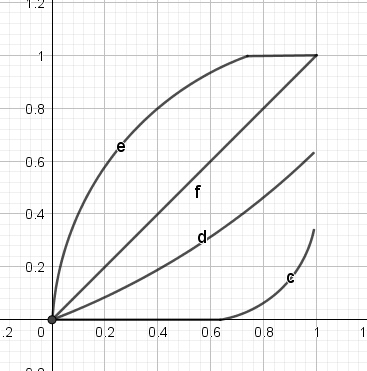
\includegraphics[width=0.2\textheight]{yurineprav.jpg}
    \label{fig:my_label}
\end{figure}

На рисунке:\\
e - сюръективная, но не инъективная;
f - биективная;\\
d - инъективная, но не сюъективная;
c - ни сюръективная, ни инъективная.

\section{Эквивалентное множество. Понятие мощности множеств.}

Пусть даны множества \textbf{A} и \textbf{B}. Если по определённому правилу каждому элементу $a \in \textbf{A}$ ставится в соответствие единственный элемент $b \in \textbf{B}$, и в силу того же правила каждому элементу $b \in \textbf{B}$ ставится в соответствие единственный элемент $a \in \textbf{A}$, то между элементами установлено \indef{взаимно однозначное соответствие}.\par

Если \textbf{A} и \textbf{B} - конечные, то установить взаимно однозначное соответствие между их элементами можно тогда и только тогда, когда число элементов у них \emph{одинаковое}.\par 

Если множество бесконечное, то можно установить взаимно однозначное соответствие между самим этим множеством и его элементами.\\
Пусть дано множество натуральных чисел $N$, $A$ - множество положительных чётных чисел. $n \leftrightarrow 2n$, устанавливается соответствие по этому новому правилу, хотя $A \in N$.

\begin{definition}
Множества \textbf{A} и \textbf{B}, между элементами которых установлено взаимно однозначное соответствие, называются взаимно однозначными множествами: $\textbf{A} \sim \textbf{B}$. 
\end{definition}

Отметим следующие свойства: 


1)$\textbf{A} \sim \textbf{A}$;


2)Если $\textbf{A} \sim \textbf{B}$, то $\textbf{B} \sim \textbf{A}$;

3)Если $\textbf{A} \sim \textbf{B}$ и $\textbf{B} \sim \textbf{C}$, то $\textbf{A} \sim \textbf{C}$.\par 

Если множества конечные, то их эквивалентность означает, что их число элементов одинаковое. Ранее мощностью конечного множества было названо число элементов этого множества. Т.е. число элементов эквивалентных множеств есть то общее, что им присуще. Поэтому естественным становится следующее определение.

\begin{definition}
\indef{Мощностью} произвольного множества \textbf{A} называется то общее, что есть у всех множеств, эквивалентных \textbf{A}. Эквивалентные множества имеют одну и ту же мощность.
\end{definition}

\section{Счётные множества.}

\begin{definition}
Множество, эквивалентное множеству $N$ натуральных чисел, называется счётным множеством.
\end{definition}

Из этого определения следует, что все элементы счётного множества можно пронумеровать(указать порядок нумерации).\par 
Отметим следующие свойства счётных множеств:
\begin{enumerate}
    
    \item Любое подмножество счётного множества либо конечное, либо счётное.
    
    
    Пусть $A$ - счётное множество, значит, его элементы можно пронумеровать, $A = \{a_1, a_2, a_3...\}$, существует подмножество $B \subseteq A: a_{n1}, a_{n2},...$.
    
    
    Если среди чисел $n_1, n_2, ...$ есть наибольшее, то подмножество $B$ - конечное. А если среди указанных чисел наибольших нет, то оно счётное.
    
    \item Объединение любого конечного или счётного числа счётных множеств --- снова счётное множество.
    
    
    Рассмотрим случай, когда объединяется счётное число счётных множеств:$A_1, A_2, A_3, A_4...$. 
    
    
    Можно считать, что эти множества не имеют одинаковых элементов, и если это так, то можно перейти к $A_1, A_2\backslash A_1, A_3 \backslash (A_1 \cup A_2), ...$, каждое из которых не счётно, и все множества не содержат одинаковых элементов.
    
    \begin{figure}[h!]
       
       \begin{center}
       
       \begin{tikzpicture}[line cap=round,line join=round,>=triangle 45,x=1.0cm,y=1.0cm]
\draw [color=cqcqcq,, xstep=2.0cm,ystep=2.0cm] (-2.5,-0.5) grid (5.,6.8);
\clip(-2.5,-0.5) rectangle (5.,6.8);
\draw [->,line width= 1 pt] (-2.,6.) -- (0.,6.);
\draw [->,line width=1pt] (0.,6.) -- (-2.,4.);
\draw [->,line width=1pt] (-2.,4.) -- (-2.,2.);
\draw [->,line width=1pt] (-2.,2.) -- (0.,4.);
\draw [->,line width=1pt] (0.,4.) -- (2.,6.);
\draw [->,line width=1pt] (2.,6.) -- (4.,6.);
\draw [->,line width=1pt] (4.,6.) -- (2.,4.);
\draw [->,line width=1pt] (2.,4.) -- (0.,2.);
\draw [->,line width=1pt] (0.,2.) -- (-2.,0.);
\begin{scriptsize}
\draw [fill=qqqqtt] (-2.,6.) circle (2.5pt);
\draw[color=qqqqtt] (-1.7501989461869456,6.450940215315453) node {$a_{11}$};
\draw [fill=black] (0.,6.) circle (2.5pt);
\draw[color=black] (0.25578127058899647,6.450940215315453) node {$a_{12}$};
\draw [fill=black] (2.,6.) circle (2.5pt);
\draw[color=black] (2.240421272292854,6.450940215315453) node {$a_{13}$};
\draw [fill=black] (4.,6.) circle (2.5pt);
\draw[color=black] (4.246401489068796,6.450940215315453) node {$a_{14}$};
\draw [fill=black] (-2.,4.) circle (2.5pt);
\draw[color=black] (-1.814219591403199,4.359599138251179) node {$a_{21}$};
\draw [fill=black] (0.,4.) circle (2.5pt);
\draw[color=black] (0.25578127058899647,4.380939353323264) node {$a_{22}$};
\draw [fill=black] (2.,4.) circle (2.5pt);
\draw[color=black] (2.2617614873649385,4.316918708107011) node {$a_{23}$};
\draw [fill=black] (4.,4.) circle (2.5pt);
\draw[color=black] (4.246401489068796,4.444959998539517) node {$a_{24}$};
\draw [fill=black] (-2.,2.) circle (2.5pt);
\draw[color=black] (-1.686178300970692,2.332278706403158) node {$a_{31}$};
\draw [fill=black] (0.,2.) circle (2.5pt);
\draw[color=black] (0.29846170073316547,2.4603199968356644) node {$a_{32}$};
\draw [fill=black] (2.,2.) circle (2.5pt);
\draw[color=black] (2.3044419175091075,2.481660211907749) node {$a_{33}$};
\draw [fill=black] (4.,2.) circle (2.5pt);
\draw[color=black] (4.246401489068796,2.4389797817635803) node {$a_{34}$};
\draw [fill=black] (-2.,0.) circle (2.5pt);
\draw[color=black] (-1.7075185160427766,0.4543397800597284) node {$a_{41}$};
\draw [fill=black] (0.,0.) circle (2.5pt);
\draw[color=black] (0.2131008404448275,0.47567999513181286) node {$a_{42}$};
\draw [fill=black] (2.,0.) circle (2.5pt);
\draw[color=black] (2.3044419175091075,0.47567999513181286) node {$a_{43}$};
\draw [fill=black] (4.,0.) circle (2.5pt);
\draw[color=black] (4.246401489068796,0.4543397800597284) node {$a_{44}$};
\end{scriptsize}

\end{tikzpicture}
   
    \end{center}
   
    \end{figure}
    
    Укажем порядок нумерации элементов в объединении этих элементов. Очевидно, что при таком подходе к нумерации элементов, каждый элемент получит единственный номер, значит, будет установлено взаимно однозначное соответствие между элементами объединения множеств $A_1, A_2, A_3...$ и множеством натуральных чисел $N$.
    
    \item Если элементы множества $A$  снабжены конечным числом индексов, каждый из которых принимает счётное число значений, то множество $A$ - счётно.
    
    \item Из свойства 3 следует свойство 4: множество рациональных чисел - счётно, $\Rightarrow \frac{p}{q}$, где и числитель, и знаменатель принимают счётное множество значений.
    
    \item Если множество $A$ - бесконечное, то из него можно выделить счётное подмножество, и оставшаяся часть при этом будет бесконечной. 
    
    
    Действительно, пусть $A$ - бесконечное множество. Выберем $a_1$ и $b_1$, отличные друг от друга. Т.к. множество бесконечно, снова можно выбрать $a_2$ и $b_2$. Аналогично $a_3$ и $b_3$ и т.д.\\
    $A_1$ и $B$ - два счётных подмножества. Очевидно, что множество $B$ содержится во множестве $A \backslash A_1$, но множество $B$ - счётное, значит и множество $A \backslash A_1$ - бесконечное: $B \subseteq A \backslash A_1 \Rightarrow A \backslash A_2$ - бесконечное. 
    
    \item Если из бесконечного множества удалить счётное подмножество, то оставшаяся часть множества будет эквивалентна исходному множеству. 
    
    
    \(\blacksquare\) \textbf{Доказательство.} 
    
    
    Пусть $M$ - бесконечное множество. По свойству 5 из этого множества можно выбрать 2 счётных подмножества $A$ и $B$. Обозначим $N = M \backslash (A \cup B)$, причём поскольку $A$ и $B$ - не пересекающиеся, то, очевидно, что $N = (M \backslash A) \backslash B$. Отсюда множества $M = N \cup (A \cup B) \Rightarrow$ $M \backslash A = N \cup B$.
    
    
    Покажем, что множество $M$ и $M \backslash A$ - эквивалентны.
    
    
    Действительно, поскольку $A$ и $B$ - счётные множества, то $(A \cup B)$ тоже счётное множество. Установим взаимно однозначное соответствие между $M \backslash A$ и $M$. 
    
    
    Пусть $x \in M \backslash A \Rightarrow x \in N \cup B$. Во множестве $M$ этому $x$ будет соответствовать он сам, если $x \in N$, и он будет соответствовать $y$, если $x \in B$, т.к. множество $B$ и $(A \cup B)$ - эквивалентны. В обратную сторону взаимно однозначное соответствие устанавливается аналогично. $x' \in M \Rightarrow x' \in N$ или $x' \in A \cup B$. Из $x' \in N \Rightarrow$, что во множестве $M \backslash A x'$ соответствует самому себе, а из $x' \in A \cup B \Rightarrow x'$ должен соответствовать $y' \in B$, т.к. множество $A \cup B$ и $B$ - эквивалентны. 
    
    
    Из доказанного свойства получаем, что если к бесконечному множеству добавить конечное или счётное множество, то вновь полученное множество будет эквивалентно первоначальному.

\end{enumerate}

\section{Сравнение мощностей множеств.}

Пусть даны \textbf{A} и \textbf{B} - два множества. Если во множестве \textbf{A} есть подмножество $\textbf{A}_1$, $\textbf{A}_1 \subseteq \textbf{A}$, $\textbf{A}_1 \sim \textbf{B}$, а сами множества \textbf{A} и \textbf{B} не эквивалентны, то мощность множества \textbf{A} больше мощности \textbf{B}, \Rightarrow |\textbf{A}|>|\textbf{B}|.


Справедлива следующая теорема Кантора-Бернштейна. 

\begin{theorem}

Если во множестве \textbf{A} есть $\textbf{A}_1 \subseteq \textbf{A}$, $\textbf{A}_1 \sim \textbf{B}$, то мощности множеств \textbf{A} и \textbf{B} --- одинаковы: $|\textbf{A}| = |\textbf{B}|$

\[ 
\begin{cases}
\mathbf{A}, \mathbf{A}_1 \subseteq \mathbf{A}, \mathbf{A}_1 \sim \mathbf{B} \\
\mathbf{B}, \mathbf{B}_1 \subseteq \mathbf{B}, \mathbf{B}_1 \sim \mathbf{A}
\end{cases}
\Rightarrow |\mathbf{A}| = |\mathbf{B}|
\]

\end{theorem}

Из этой теоремы следует, что если есть 2 произвольных множества \textbf{A} и \textbf{B}, то для них выполняется одно из условия: 

\begin{enumerate}
    
    \item |\textbf{A}| > |\textbf{B}|;
    
    \item |\textbf{A}| < |\textbf{B}|;
    
    \item |\textbf{A}| = |\textbf{B}|.

\end{enumerate}


\section{Существование несчётных множеств. Теорема Кантора}


\begin{theorem} 

Множество точек отрезка [0,1] несчётно.

\end{theorem}

\(\blacksquare\) \textbf{Доказательство от противного:}

Предположим, что множество точек отрезка [0,1] счётно. Тогда каждую точку можно пронумеровать. Получим последовательность $x_1, x_2, ... , x_m$. Разделим отрезок
[0,1] на 3 равные части. Тогда по крайней мере одна из этих частей не будет содержать точку $x_1$ (если бы мы делили на 2 части, то был бы возможен случай, когда эта точка лежит на правом конце первой части и на левом конце второй части, то есть принадлежит обоим частям). Этот отрезок обозначим $\Delta_1$: $x_1 \notin \Delta_1$. Полученный отрезок так же поделим на 3 части, получим $\Delta_2$:  $x_2 \notin \Delta_2$. Аналогичным образом $\Delta_3$, ... , $\Delta_m$. В результате возникает последовательность вложенных друг в друга отрезков, длины которых стремятся к 0. Из теоремы о вложенных отрезках $\Rightarrow \exists x_0 \in$ всем отрезкам $\Delta_1$, ... , $\Delta_m$ $\Rightarrow x_0$ не может совпадать ни с одной из точек отрезка $x_1, ... , x_m \in$[0,1]. При этом $x_0 \in$[0,1] $\Rightarrow$ точка $x_0$ должна совпадать с одной из точек $x_1, ... , x_m$. Получили противоречие $\Rightarrow$ множество точек отрезка [0,1] несчётно.

\section{Множество мощности континуум.}

\begin{definition}

Множества, эквивалентные множеству точек [0;1], называются множествами мощности континуум или континуальными множествами.

\end{definition}

Из теоремы Кантора и других следует, что множество мощности континуум имеют мощность больше мощности счётных множеств. \par

Отметим следующие \underline{свойства}:

\begin{enumerate}
    
    \item Множество точек любого отрезка [a,b] - множество мощности континуум. Это следует из того, что между точками отрезка [0;1] и [a,b] можно установить взаимно однозначное соответствие. 
    
    
    $y = a + (b-a)x, x \in [0;1]$
    
    
    $x = \frac{y - a}{b - a}, \hspace{1mm} \textrm{если} \hspace{1mm} y \in [a,b]$.
    
    \item Т.к. добавление конечного числа элементов к бесконечному множеству не меняет его мощность, то мощность множества точек [a,b), (b,a] и (a,b) - это множество мощности континуум.
    
    \item Множество точек числовой прямой - это множество мощности континуум. Действительно, это следует из того, что между $(-\frac{\pi}{2}; \frac{\pi}{2})$ и $(-\infty ; \infty)$ можно установить взаимно однозначное соответствие по формуле $y = \tan (x)$.
    
    \item Множество иррациональных чисел отрезка [0;1] и любого другого --- это множество мощности континуум $\Rightarrow$ иррациональных чисел больше, чем рациональных чисел, так как последние счётны.
    
    \item Объединение счётного числа множеств мощности континуум снова множество мощности континуум.
    
    \item Объединение континуума множеств, каждое из которых множество мощности континуум, снова будет множество мощности континуум. 

\end{enumerate}

\section{Существование множеств со сколь угодно большими мощностями.}

\begin{theorem}

Множество всех подмножеств непустого множества имеет мощность большую, чем мощность самого множества.

\end{theorem}

\(\blacksquare\) \textbf{Доказательство.}


Пусть дано множество $M, m$. Множество всех подмножеств множества $M$ обозначим за $T, t$. Отметим, что множество $T$ в качестве элементов содержит пустое множество $\varnothing$ и $M$. 


Очевидно, что во множестве $T$ есть подмножество $T_0 \sim M$, $T_0 \subseteq T$. $T_0$ - это одноэлементные подмножества множества $M$.


Предположим, что между элементами множеств $T$ и $M$ можно установить взаимно однозначное соответствие. Тогда разобъём все элементы множества $M$ на 2 класса:


\textbf{1 класс} - те элементы множества $M$, которые входят в соответствующие ему подмножества из $T$.


Так, например, к \textbf{1 классу} будет отнесён элемент $m' \in M$, который соответствует элементу $t' = M \subseteq T$.


Ко \textbf{2 классу} отнесём те элементы множества $M$, которые входят в соответствующее подмножеству $T$. 


Так, например, ко \textbf{2 классу} будет отнесён $m'' \in M$, который соответствует элемент $t'' = \varnothing \subseteq T$.


Таким образом, оба эти класса непустые и, очевидно, что каждый элемент множества $M$ попадает только в один из классов. 


Рассмотрим все элементы множества $M$, принадлежащие 2 классу. Это будет подмножество множества $M$,и, значит, это будет элементы множества \textbf{T}. Во множестве $M$ существует элемент $m_0 \in M$, который соответствует множеству элементов 2 класса, как элемент множества \textbf{T}. Выясним, какому классу принадлежит элемент $m_0$.


Предположим, что $m_0 \in \hspace{1mm} \textrm{1 классу}$, т.е. $m_0$ входит в соответствующее ему подмножество из множества $M$, но это невозможно, т.к. соответствующее ему подмножество множества $T$ состоит из элементов 2 множества.


Предположим, что $m_0 \in \hspace{1mm} \textrm{2 классу}$, т.е. не входит в соответствующее ему подмножество из множества $T$, но это тоже невозможно, т.к. во 2 классе уже собраны все элементы, ему принадлежащие.


Таким образом, $m_0$ не попадает ни в 1 класс, ни во 2 класс, чего быть не может. Полученное противоречие указывает на то, что наше предположение об эквивалентности $M \sim T$ неверно. Значит, $M$ и $T$ не эквивалентны. Это означает, что мощность множества $T$ больше мощности множества множества $M$. Теорема доказана.

\(\square\) \textit{Замечание.}


Не существует множества с наибольшей мощностью (аналогично тому, что не существует самого большого натурального числа).


\begin{figure}[h!]
  \centering
    
    
\includegraphics[width=0.12\textheight]{goblin-puchkov.jpg}
    \label{fig:my_label}

\end{figure}




\section*{\textbf{Раздел II}}


\section{Предмет комбинаторики}

\indef{Комбинаторика} - это раздел дискретной математики, в котором решаются задачи, связанные с выбором элементов, как правило, из конечного множества и расположения их в соответствии с заданными правилами. \par 
Каждое такое правило позволяет построить конструкцию из элементов данного множества. Такая конструкция называется \indef{комбинаторной конфигурацией.} \par 
Задачами комбинаторного анализа являются разработка алгоритмов построения комбинаторных конфигураций и конфигурация этих алгоритмов. \par 
Число современных задач, решаемых комбинаторными методами относятся: 

\begin{enumerate}
    
    \item Задачи на размещение на плоскости некоторых плоских фигур с указанными свойствами;
    
    \item Задачи на заполнение некоторых пространственных тел меньшими телами с указанными объёмами и конфигурацией;
    
    \item Задачи на кратчайшие пути;
    
    \item Задачи компьютерных, транспортных и электрических сетей и многое другое.

\end{enumerate}

Отметим, что основными операциями над множествами в комбинаторном анализе являются две операции: отбор элементов из множества и упорядочение их по заданным правилам.\par 
К числу простейших комбинаторных конфигураций относится размещение, перестановки, сочетания множеств и др. При подсчёте их числа используются два правила: правило суммы и правило произведения.

\section{Правило суммы и правило произведения.}


\indef{Правило 1}(правило суммы).\par
Пусть дано некоторое множество \textbf{S}, и из этого множества подмножество \textbf{A}(оно может состоять из одного элемента) можно выбрать m способами, а подмножество \textbf{B} можно выбрать n способами, причём эти выборы таковы, что их нельзя осуществить одновременно, то тогда выбрать $\textbf{A} \cup \textbf{B}$ из множества \textbf{S} можно m+n способами.\par 

\underline{Пример.} Есть 100 деталей - 60 штук 1-го сорта, 30 штук 2-го сорта, 10 - 3-го сорта. Тогда выбрать детали 1-го и 2-го сорта есть 60 + 30 = 90 способов.

\indef{Правило 2}(правило произведения). \par 
Пусть из множества \textbf{S} подмножество \textbf{A} можно выбрать m способами. После этого, подмножество \textbf{B} можно выбрать n способами. Тогда $\textbf{A} \cup \textbf{B}$ можно выбрать $m \cdot n$ способами. Отметим, что правило произведения на практике часто используется в следующей формулировке: \par 

Пусть 1-е действие можно выполнить n способами, после этого 2-е действие - $n_2$ способами и тогда k-е действие можно выполнить $n_k$ способами. То тогда выполнить все n указанных действий можно $n_1 \cdot n_2 \cdot n_3 \cdot \dots \cdot n_k$ способами. \par 

\underline{Пример.} Сколько существует пятизначных чисел? 
Так как на 1 месте в пятизначном числе не может стоять 0(т.к. тогда бы это было четырёхзначное число), то выбрать первую цифру на 1 место можно 9-ю способами(это может быть 1,2,3,4,5,6,7,8,9). Выбрать 2, 3, 4, 5 место можно выбрать 10-ю способами(это может быть 1,2,3,4,5,6,7,8,9 или 10). Значит, всего существует $9 \cdot 10^4 = 90000$ способов.


\section{Размещение.}


\subsection{Размещение без повторения.}

Есть множество s  из n различных элементов, будем выбирать из него по одному последовательно k элементов 0 < k < n каждый элемент перед отбором следующего не возвращается в s Такой отбор называется размещение из n элементов по k. 

То есть это такие комбинации из этих n элементов, каждая из которых содержит в точности k элементов и отличаются эти комбинации одна от другой либо составом либо порядком элементов при этом предполагается, что все n элементов множества s - различные. 

(*)$A_n^k = n (n-1) \dots (n-(k - 1))$ - общее число размещений из n элементов по k 

1-ый - можно выбрать n способами, 2-ой - (n-1) способами, \dots k-ый (n-(k-1))- способами, тогда по правилу произведения получим на лицо формулу(*)

\underline{Пример}:

16 команд в турнире. Сколько вариантов распределить призовые места:

$A_n^K = A_{26}^3 = 16*15*14$

\subsection{Размещение с повторениями.}

Снова есть множество из n элементов. Отбираем из него k<n элементов. 

Но теперь каждый отобранный элемент перед отбором следующего возвращается в множество S. 

Это будет размещением из n элементов по к с повторениями.



Общее число размещений с повторениями обозначаем, как $\hat{A}_n^k$
%нормальное обозначение

Получаем формулу: 1-ый - n способами, 2-ой - n  способами \dots k-ый -n способами, тогда, по правилу произведения  $\hat{A}_n^k = n^k$

\underline{Пример}:

Сколько трехзначных чисел можно составить из чисел 1,2,3,4


%1-ая - 4 способами, 2-ая - 4 способами, 3-ая - 4-способами

N= $\hat{A}_n^k = n^k$ = $4^3$ = 64

\section{Перестановки.}



\subsection{Перестановки без повторений.}

Пусть есть множество S, состоящее из n элементов k=n, тогда из множества S отбираются все его элементы. И значит одна комбинация от другой  может отличаться только порядком элементов.

То есть перестановки из n различных элементов это такие комбинации из этих элементов, каждая из которых содержит все n элементов.

$P_n=n!$

%комментарий

$P_n = A_n^k = n(n-1)(n-2)\dots(n-(n-1)) = n!$

\subsection{Перестановки с повторениями.}

Во множество S n элементов, среди них есть одинаковые элементов первого типа $n_1$, второго $n_2$, \dots k-ого $n_k$. Так что $n_1+n_2+\dots +n_k=n$

Перестановки с повторения будем обозначать так: $P_n(n_1,n_2,\dots ,n_k)$

Возьмём любую из перестановок этих n элементов. В ней элементы первого типа можно переставит $n_1!$ раз при этом перестановка не изменится. Элементов второго $n_2!$ и так далее к-ого $n_k!$ и ничего не изменится. Если б все элементы были разными, то $P_n=n!$

Теперь их будет меньше в $n_1!n_2!\dots n_k! \xRightarrow[]{} P_n(n_1,n_2,\dots, n_k) =  \frac{n!}{n_1!n_2!\dots n_k!} $

\section{Сочетания.}

\subsection{Сочетания без повторений.}

Сочетанием из n по k элементов называются такие комбинации из этих n элементов, каждая из которых содержит k Элементов и отличается одна комбинация от другой только составом элементов

Возьмем сочетание из n по k, переставим в ней элементы всевозможными образом, получим k! комбинаций. 

Получим размещение $A_n^k$ $C_n^k \cdot k! = A_n^k \xRightarrow[]{} С_n^k = \frac{A_n^k}{k!} = \frac{n!}{k!(n-k)!}$

\underline{Пример}:

Из группы в 10 человек надо выделить 3 для работы
$C_{10}^3 =  \frac{10!}{3!7!} = \frac{8\cdot 9 \cdot 10}{6} = \frac{8 \cdot 3 \cdot 5}{1} = 120$

\subsection{Сочетания с повторениями.}

Если в сочетании элементы могут повторяться, то такие сочетания называются сочетаниями с повторениями из n элементов по k.

Можно показать, что общее число сочетаний с повторениями из n по k находятся по формуле $\hat{C}_n^k = С_{n+k-1}^k$

\underline{Пример}:

Есть 4 вида пирожных. Сколько разных вариантов при покупке 7 пирожных. 

$\hat{C}_4^7 = С_{4+7-1}^7 = С_{10}^7=120$




\underline{Замечание}: 

\begin{enumerate}
    \item Множество как правило конечное 
    \item Основными операциями над элементами множества являются отбор и упорядочение их
    
\end{enumerate}

\section{Разбиение множества на группы.}

Пусть есть множество S, состоящее из N различных элементов. Подсчитаем сколько есть вариантов разбиения этого множества S на K упорядоченных подмножеств $S_1,S_2, \dots ,S_k$  можно рассмотреть как последовательность их расположения. Первое подмножество $S_1$, содержащее $n_1$ элементов выбираем из множества S, состоящего из n элементов $С_ {n}^{n_1}$ 

После этого выбираем подмножество $S_2$ из $S(n-{n_1})$ элементов $C_{n-{n_1}}^{n_2} $, теперь выбираем подмножество $S_3$ Из $S(n-{n_1}-{n_2})$ элементов. 

$C_{n-{n_1}-{n_2}}^{n_3} $

\dots

Подмножество $S_k$ состоящее из $n_k$ элементов из $S(n-{n_1}-{n_2}\dots -{n_{k-1}}$  

$C_{n-{n_1}-{n_2}- ...-{n_{k-1}}}^{n_k} $

Тогда по правилу произведения получаем, что выбрать подмножества 

$S_1, \dots , S_k$ из S в указанном порядке можно следующим числом способов:


$C_{n}^{n_1} $
\cdot$C_{n-{n_1}}^{n_2} $
\cdot$C_{n-{n_1}-{n_2}}^{n_3} $
\dots \cdot$C_{n-{n_1}-{n_2}- ...-{n_{k-1}}}^{n_k} $= $\frac{n!}{n_1,n_2,\dots n_k}$

Столько вариантов разбиения множества S состоящего из n различных элементов на k упорядоченных подмножеств непустых и не пересекающихся с числом элементов $n_1,n_2 \dots n_k$

$N(n_1,n_2,\dots n_k)$ - число разбиений

$N(n_1,n_2,\dots n_k) = \frac{n!}{n_1,n_2,\dots n_k}$

\underline{Пример}:

В группе шли выборы старосты, за предложенную кандидатуру проголосовало 15, и 5 против, 5 воздержались. Сколько вариантами могли быть проведены выборы?

$N(15,5,5) = \frac{25!}{15!\dot5!\dot5!}$

\section{Определение числа элементов в объединении нескольких элементов.}

\subsection{Метод включения и исключения.}

Этот метод применяется в задаче, когда рассматриваемое множество надо разбить на подмножества в зависимости от того, обладают ли его элементы определенными свойствами. 

Определение числа элементов в объединении нескольких множеств:

Даны множества A и B
n(A), n(B) 
$n(A \cup B) -?$ 

$n(A\cup B) = n(A) + n(B), если A \cap B =   \emptyset$

$A\cap B \neq \emptyset, то n(A\cup B) = n(A) + n(B) - n(A\cap B)$

%картинка 

Посчитаем число элементов в объединении 3-ех множеств: 

$n(A\cup B\cup C) = n(A) + n(B) + n(C) - n(A \cap B) - n(A \cap C) - n(B  \cap C) + n(A \cap B \cap C)  $

$n(A\cup B\cup C) = n[A\cup \textbf{(B\cup C)}] = n(A) + n(B\cup C) - n(A\cap(B \cup C)) = n(A) + n(B) + n(C) - n(B\cap C) - n(A\cap B) - n(A \cap C) + n((A\cap B)+ (A\cap C)) = n(A) + n(B) + n(C) - n(A\cap B) - n(A\cup C) - n(A\cap B \cap C)$

Если объединяется k множеств, то число элементов в их объединении находится по формуле:

$n( \cup_{i=1}^k A_i) = \sum_{i=1}^k n (A_i) - n(A_1 \cap A_2\cap \dots \cap A_k) $

(*)

\underline{Следствие}:

Пусть есть множество $A,A_1,\dots A_k $ - подмножество множества A. Тогда число элементов множества A, не принадлежащих на одному из множеств $A,A_1,\dots A_k $ находится по формуле:

$N= n(A) - (n(A_1)+\dots +n(A_k)) + (n(A_1 \cap A_2) + n(A_1 \cap A_3)+ \dots n(A_{k-1} \cap A_k) + \dots  (-1)^{k-1} n(A_1\cap A_2\dots  \cap A_k) + \dots +(-1)^{k-1} n(A_1 \cap A_2 \dots \cap A_k)   $ 
%формула (1)

Формула (1) непосредственно следует из равенства (*)

\underline{Пример}

Все, кто работает в лаборатории знают хотя бы один иностранный язык.

Английский - 12 человек, Немецкий - 8 человек,Французский - 7 человек,Английский и немецкий - 5 человек, Английский и Французский - 4 человека, немецкий и французский - 3 человека, все 3 языка - 2 человека

Сколько всего человек работает в лаборатории.

$n(A\text{А}\cup A\text{Н} \cup A\text{Ф} ) = n(A\text{А}) + n(A\text{Ф}) + n(A\text{Н}) - n(A\text{А}\cap A\text{Н}) + n(A\text{А}\cap A\text{Ф})+
n(A\text{Ф}\cap A\text{Н}) + n(A\text{А}\cap A\text{Н}\cap A\text{Ф}) = 12 + 8 + 7 -(5 + 4 +3) + 2 = 29 - 12 = 17$

\subsection{Определение числа элементов множества не обладающего ни 1 из свойств.}

Пусть есть некоторое множество, состоящее из N элементов и n свойств  $P_1,P_2,\dots P_n$ совместимых друг с другом.

Число элементов этого множества, обладающих свойствами $P_i1,P_i2,\dots P_ik$(обозначим $N i1,i2,\dots ik$) и может быть некоторыми другими

Число N(0) элементов данного множества, не обладающих ни одним из свойств $P_1,P_2, \dots P_n$ находится по следующей формуле:

$N(0)= N - S_1 + S_2 - S_3 + \dots +(-1)^n S_n$(*), где 
$S_1$
- число элементов обладающих одним свойством:

$S_1 = N_1 + N_2 + \dots N_n$

$S_2 = N_12 + N_13 + \dots N_{{n-1}_n}$- Обладающих 2 свойствами

$S_3$- Обладающих 3 свойствами

И так дальше

Эта формула непосредственно следует из формулы предыдущего пункта

\underline{Пример}

S - Множество целых чисел от 1 до 100 

$P_1$ делится на 2, $P_2$ делится на 3, $P_3$ делится на 5, тогда число чисел от 1 до 100, не делящихся ни на 2, ни на 3, ни на 5

Найдем по формуле N(0) = N -$S_1 + S_2 - S_3$

$S_1 = N_1 + N_2 + N_3$

$N_1 $- число чисел от 1 до 100 обладающих свойством $P_1$



$N_1 = [\frac{100}{2}]=50$
$N_2 = [\frac{100}{3}]=33$
$N_3 = [\frac{100}{5}]=20$

$S_2 = N_12 + N_13 + N_23$

$N_12 =[\frac{100}{6}]=16$ 
$N_13 =[\frac{100}{10}]=10$
$N_23 =[\frac{100}{6}]=16$

$S_3 = N_123$

$N_123 = [\frac{100}{30}] = 3$

N(0) = 100 - 103 - 32 -3 = 26
\subsection{Определение числа элементов множества, обладающего определенным набором свойств.}

N,n - свойства $P_1,P_2,\dots P_n$, совместимых друг с другом. Обобщая формулу(*) можно получить формулу для числа элементов этого множества, обладающего ровно r свойствами из n (1 $\leq$ r $\leq$ n)

$N(r)= C_r^r \cdot S(r) - C_{r+1}^r \cdot S(r+1) + C_{r+2}^r \cdot S(r+2)- \dots (-1)^{n-r} C_n^r \cdot S(n)$ (1)

S(r) - число элементов данного множества, обладающего r - свойствами

\dots

S(r+1) - r+1 свойством и так дальше

\underline{Пример}

Сколько целых от 1 до 500 $\vdots$ 3,5 или 7

$P_1 \vdots 3, P_2 \vdots 5, P_3 \vdots 7$

$N(1) = C_1^1 S(1) - C_2^1 S(2) + C_3^1 S(3)$ 

$N_1 = [\frac{500}{3}] = 166$
$N_2 = [\frac{500}{5}] = 100$
$N_3 = [\frac{500}{7}] = 71$

$S(1) = N_1 + N_2 + N_3 = 166 + 106 + 71 = 337$

$N_{12}= [\frac{500}{15}]=33$
$N_{13}= [\frac{500}{21}]=23$
$N_{23}= [\frac{500}{35}]=7$

$S(2) = N_{12} + N_{13} + N_{23}= 33 + 23 + 7 = 70$ 


$S(3) = N_{123} = [\frac{500}{105}] = 4$

Учитывая это находим: $N(1) = C_1^1 S(1) - C_2^1 S(2) + C_3^1 S(3) = 337 - 140 + 12 = 209$

\section{Бином Ньютона и полиномиальная формула.}

\subsection{Бином Ньютона.}


$(a+b)^n = \sum\limits_{k=0}^n  C_{n}^{k} \cdot a^k b^{n-k}$

\(\blacksquare\)\textbf{Доказательство (методом математической индукции):}\\

1. Докажем при n = 1 (база индукции):

$(a+b)^1 = \sum\limits_{k=0}^1  C_{1}^{k} \cdot a^k b^{1-k} = C_{1}^{0}a^0b^1 + C_{1}^{1}a^1b^0 = b + a$

2. Переход: предположим, что верно при n-1, то есть $(a + b)^{n-1} = \sum\limits_{k=0}^n  C_{n-1}^{k} \cdot a^k b^{n-1-k}$

3. Докажем, что верно при n:

$(a+b)^{n} = (a+b)^{n-1}(a+b) = \sum\limits_{k=0}^{n-1} C_{n-1}^{k} a^k b^{n-1-k} \cdot (a+b) = \sum\limits_{k=0}^{n-1} C_{n-1}^{k} a^{k+1} b^{n-1-k}(\sum_1) \cdot \sum\limits_{k=0}^{n-1} C_{n-1}^{k} a^k b^{n-k}(\sum_2) $

$\textrm{В} \sum_1 \text{ заменяем индекс суммирования } {k={j-1}},$ 

$\sum_1=\sum\limits_{j=1}^{n}  C_{n-1}^{j-1} \cdot a^{j} b^{n-j} \text{ после преобразуем индекс суммирования }  \sum_1 = \sum\limits_{k=1}^{n}  C_{n-1}^{k-1} \cdot a^k b^{n-k}$

\textrm{Учитывая это:}

$(a+b)^n = \sum\limits_{k=1}^{n}  C_{n-1}^{k-1} \cdot a^{k} b^{n-k} + \sum\limits_{k=0}^{n-1}  C_{n-1}^{k} \cdot a^{k} b^{n-k}$

Выравниваем индексы суммирования, сделаем их от 0 до n одинаковыми. Для этого добавим нулевые сочетания:
$C_{n-1}^1=0$ в начало $\sum_1$, $C_{n-1}^n = 0$ в конец $\sum_2$, получим:

$\sum\limits_{k=0}^{n} C_{n-1}^{k-1} a^k b^{n-k} +  \sum\limits_{k=0}^{n} C_{n-1}^{k} a^k b^{n-k}  = \sum\limits_{k=0}^n  a^k b^{n-k} \cdot (C_{n-1}^{k-1} + C_{n-1}^{k}) \text{, то есть}$ 

$(a+b)^n =  \sum\limits_{k=0}^n  a^k b^{n-k} \cdot (C_{n-1}^{k-1} + C_{n-1}^{k} ) (*)$



\textrm{Вычислим:}
$C_{n-1}^{k-1} + C_{n-1}^{k}= \frac{(n-1)!}{(k-1)!(n-k)!} + \frac{(n-1)!}{(n-1-k)!(k)!}= \frac{(n-1)!}{(k-1)!(n-k-1)!}(\frac{1}{k}+ \frac{1}{n-k}) = \frac{(n-1)!}{(k-1)!(n-k-1)!} \cdot \frac{n}{(n-k)k} = \frac{n!}{k!(n-k)!} = C^{k}_n \textrm{ (подставим это в равенство *)}
$

{$\Longrightarrow$}
\[(a+b)^n =\sum\limits_{k=0}^n  C_{n}^{k} \cdot a^k b^{n-k}
\]




Бином Ньютона - основа для многих комбинаторных формул.

\begin{enumerate}

    \item $a = 1, b = 1,$
    
    $2^n=\sum\limits_{k=0}^n C_{n}^{k} = C_{n}^{0} +C_{n}^{1} + C_{n}^{2} + ... + C_{n}^{n}$,
    
    то есть сумма биномиальных коэффициентов $C_{n}^{k} = 2^n$
    
    * С точки зрения теории множеств эта формула означает, что число всех подмножеств множества, состоящего из n элементов = $2^n$ или мощность множества всех подмножеств, состоящего из всех элементов = $2^n$
    
    
    \item  $a = 1, b = -1:$ $\sum\limits_{k=0}^n C_{n}^{k} (-1)^{n-k} = 0$
    
    $a = -1, b = 1:$
    $\sum\limits_{k=0}^n C_{n}^{k} (-1)^{k} = 0$
    
    А это означает, что сумма биномиальных коэффициентов, стоящих на четных и нечетных позициях одинакова и каждая из них равна $2^{n-1}$
    
    * Это замечание следует из предыдущей  формулы
    
\end{enumerate}

Отметим еще некоторые свойства биномиальных коэффициентов:

\begin{enumerate}

\item $C_{n-1}^{k-1} + C_{n-1}^{k} = C_{n}^{k} $

\(\blacksquare\) Доказательство было приведено при доказательстве бинома Ньютона% Гиперссылочку?

\item $C_{n}^{n-k} = C_{n}^{k}$ - Биномиальные коэффициенты одинаково удаленные от начала(конца) разложения равны между собой

\(\blacksquare\) Проведите доказательство самостоятельно, разложив сочетания по формуле.

\end{enumerate}

\subsection{Полиномиальная формула.}

Обобщение бинома Ньютона для нескольких слагаемых(>2) является полиномиальной формулой:
\[
(a_1 + a_2 + ... + a_k)^n = \sum\limits_{\substack{r_1\geq 0,r_2\geq 0...r_k\geq 0 \\ r_1+r_2+...+r_k=1 }} \frac{n!}{r_1!r_2!...r_k!} a_1^{r_1} a_2^{r_2} \dotsc a_k^{r_k}
\]



Здесь суммирование ведется по целым неотрицательным решениям уравнения $r_1+r_2+...+r_k=1$ 

$\geq$

\section{Линейные однородные рекуррентные уравнения}

Пусть дана числовая последовательность $a_n$

\begin{definition}
\indef{Рекуррентным уравнением} называется соотношение вида $\mathbf{a_{n+k} = F(n,a_n,a_{n+1}, ..., a_{n+k-1})}$, которое выполняется при всех значениях $n$ и некоторых $k$, 
и позволяющая найти все члены числовой последовательности, если известны её первые $k$ членов.
%Например a_n_+_1 = a_n + d - формула члена арифметической прогрессии
\end{definition}
\begin{definition}
Если рекуррентные соотношение имеет вид:

$ a_{n+k} + P_1a_{n+k-1} + ... +P_ka_n = 0$ (1)%тут бы гиперссылку организовать потом

То оно называется линейным однородным рекуррентным уравнением .

Здесь  $P_1,...,P_k$ - действительные числа.
\end{definition}

Всякая числовая последовательность, удовлетворяющая(1), называется решением. Совокупность всех числовых последовательностей, удовлетворяющих(1), называется общим решением этого уравнения.

Отыскание общего решения(1) тесно связано с многочленом $P(\lambda)= \lambda^k + P_1*\lambda^{k-1} + P_2*\lambda^{k-2} + ... + P_k$, который называется характеристическим многочленом для числовой последовательности $a_n$, удовлетворяющей рекуррентному соотношению (1). 

Структура общего решения уравнения (1) описывается следующей теоремой.

\begin{theorem} 

\begin{enumerate}
\item Если $\lambda$ - действительный корень характеристического многочлена, то последовательность \{$C\lambda^n$\} - решение уравнения (1), где $C \in R$.
\item $\lambda_1, ... , \lambda_k$ - действительные и различные корни характеристического многочлена, то общим решением уравнения(1) будет \indef{$a_n=c_1 \lambda_1^n+ ... +c_k \lambda_k^n $}(2)
\item Корни характеристического многочлена различны и существует корень $*\lambda_i$ кратности r, Тогда формуле (2) будет соответствовать \indef{$a_n=(c_{i1}+c_{i2} n+c_{i3} n^2+ ... +c_k n^{r-1}) \lambda_i^n $}
\end{enumerate}

\end{theorem}

Сформулированная теорема позволяет получить решения уравнения(1). Если будут заданы начальные условия, то они позволят определить  значения постоянных $C_1,..., C_k$ и тем самым указать конкретное решение уравнения(1)

\underline{Пример}:

$a_{n+2} - 4 a_{n+1} + 4 {a_n} = 0$ 

$a_0 = 4 , a_1 = 10$

\begin{enumerate}
    \item Составим характеристический многочлен, удовлетворяющий данному уравнению
    
    $P(\lambda) = \lambda^2 - 4  \lambda + 4$

    \item Найдем корни характеристического уравнения:
    
    $\lambda^2 - 4\lambda + 4 = 0$
    
    $\xRightarrow[]{\text{решаем квадратное уравнение} } $ 
    
    $\lambda_1 = 2, \lambda_2 = 2 $

    \item С использованием пунктов 2 и 3 сформулированной теоремы получаем 2 слагаемых:
    
    $ a_n = (C_1 + C_2 \cdot n) \cdot 2^n  $ - общее решение заданного рекуррентного уравнения, где $ C_1, C_2 \in R$
    
    \item Используя начальные условия $(a_0 = 4, a_1 = 10), $ определим значения постоянных $С_1 + С_2$
    
    Для этого в общее решение, подставим n=0
    
    Получим $a^0=(C_1 +C_2 \cdot 0) \cdot 2^0$
    
    $\Rightarrow$
    
    $C_1=4$
    
    Подставим в общее решение n=1
    
    $a_1 = (C_1 + C_2 \cdot 1) \cdot 2 
    \Rightarrow C_1 + C_2=5 \Rightarrow
    \begin{cases}
         C_1 = 4 \\ 
         C_2 = 1 \\
    \end{cases}
    $
    
    \item Запишем искомое решение заданного уравнения. Для этого в общее решение подставим $C_1 = 4, c_2 = 1$
    
    Получим 
    
    $a_n = (4+n) \cdot 2^n$

    
    

\end{enumerate}



\section{Линейные неоднородные рекуррентные уравнения.}

Линейное неоднородное рекуррентное уравнение имеет вид: 

$a_{n+k}+P_1  a_{n+k-1}+ ... + P_1a_{n} = f(n)$ (*)

f(n) - функция натурального аргумента

Отыскание общего решения уравнения (*) базируется на следующей теореме:

\begin{theorem}

Общее решение неоднородного уравнения(*) равно суме общего решения соответствующего однородного уравнения  и какого-либо частного решения (конкретного) данного неоднородного уравнения(*) 

\textbf{$a_n = a_n$(однородное)$ + {a_n}^*$} (**) 

${a_n}^*$ - частное решение неоднородного уравнения(*)

$a_n$(однородное) - общее решение соответствующего однородного уравнения (1) 

\end{theorem}

Из этой теоремы следует, что нужно научиться находить какие-либо решения данного неоднородного уравнения.

В некоторых случаях по виду правой части (*) можно указать вид частного решения неоднородного уравнения с неопределенными коэффициентами, а потом их найти 

Рассмотрим эти случаи :

\subsection{Решение уравнений вида: \texorpdfstring{$f(n) = A \beta^n$}{Lg}.}

$a_{n+k}+P_1  a_{n+k-1}+ ... + P_1 a_{n} = A \beta^n; A,\beta$ \in R

В этом случае  частное решение принимает вид:

\[ 
    \textbf{${a_n}^*$ = }
    \begin{cases}
         \lambda \beta^n, &\quad\text{если }  
         \beta \text{ - не корень характеристического многочлена}\\
        
        \lambda n ^ k \beta^n ,  &\quad\text{если }   \beta  \text{-  корень характеристического многочлена кратности k}\\
    \end{cases}
\]

\underline{Пример решения уравнения вида: \texorpdfstring{$f(n) = A \beta^n$}{Lg}}:

$a_{n+2} - 3 a_a{n+1} + 2 a_n = 12 \cdot 2^n$

\begin{enumerate}

    \item Находим общее решение соответствующего однородного уравнения
    
    $a_{n+2} - 3 a_a{n+1} + 2 a_n = 0 $
    
    \begin{enumerate}
        \item Составим характеристический многочлен:
        
        $P(\lambda) = \lambda ^2 + 3 \lambda + 2 $
        
        \item Найдем корни 
        
        $\lambda^2 - 3 \lambda + 2 = 0
        \xRightarrow[]{}
        \lambda_1 = 1, \lambda_2 = 2$
        
        
        
        \item Записываем общее решение  соответствующего однородного уравнения.
        
        $a_n \text{однородное} = C_1 \lambda_{1}^n + C_2 \lambda_{2}^n$
        
        $a_n \text{однородное} = C_1 {1}^n + C_2 {2}^n = C_1 + C_2 \cdot {2}^n $
    
    \end{enumerate}
    
    
    
    \item Укажем вид частного решения $a_n^*$ данного неоднородного уравнения 
    
    $\beta = 2,\text{а } \lambda_2 = 2 $, значит $\beta$ - корень характеристического многочлена кратности k= 1. 
    
    Значит $a_n^* = \alpha \cdot n \cdot 2^n $ - вид частного решения данного уравнения.(Здесь $\alpha$ - коэффициент подлежащий определению). 
    
    \item Определим коэффициент $\alpha$.
    
    Для этого находим
    
    $a_{n+1}^*= \alpha (n+1) \cdot 2^{n+1} $
    
    $a_{n+2}^*= \alpha (n+2) \cdot 2^{n+2}$
    
    Подставляем в первоначальное уравнение вместо  $a_{n+2} a_{n+2}^*, a_{n+1} a_{n+1}^*, a_{n} a_{n}^*$:
    
    Получим: $(4 \alpha n +8 \alpha)\cdot 2^n - 3(2 \alpha n + 2 \alpha) \cdot 2^n + 2 \alpha n \cdot  2^n = 12 \cdot  2^n    $
    
    $(4 \alpha n +8 \alpha) - 3(2 \alpha n + 2 \alpha)  + 2 \alpha n  = 12  $ $ \xRightarrow[]{} 2 \alpha = 12 \xRightarrow[]{} \alpha = 6$
    
    
    Подставим $\alpha = 6$ в равенство $a_n^* = \alpha  n 2^n  \xRightarrow[]{}  a_n^* = 6  n 2^n $
    
    \item Находим общее решение данного неоднородного уравнения ($a_n = a_n$ $\text{однородное} +$ $a_n^*$)
    
    Ответ: $a_n = c_1 + c_2$ $\cdot 2^n + 6 n \cdot$ $2^n$
 
\end{enumerate}



\subsection{Решение уравнений вида: f(n) = P(n).}

$a_{n+k}+P_1  a_{n+k-1}+ ... + P_1 a_{n} = P(n);P(n)$- многочлен от n

В этом случае  частное решение принимает вид:

\[ \textbf{${a_n}^*$ = }
    \begin{cases}
        Q(n), &\quad\text{если 1 - не корень характеристического многочлена}\\
        
        Q(n) n ^ k  ,  &\quad\text{если  1  -  корень характеристического многочлена кратности k}\\
    \end{cases}
\]  
    Q(n) - многочлен от n той же степени, что и P(n), причем многочлен Q(n) записывается в общем виде с неопределенными коэффициентами, которые следует определить.

\underline{Примеры определения Q(n) по P(n).}

P(n) = $n^3$ \( \Longrightarrow \) \\Q(n) = $d_0 + d_1 n + d_2 n^2 + d_3 n^3 $

P(n) = $1791  n^3$ \( \Longrightarrow \) \\Q(n) = $d_0 + d_1 n + d_2 n^2 + d_3 n^3 $

P(n) = n  \( \Longrightarrow \) \\Q(n) = $d_0 + d_1 n$

\underline{Пример решения уравнения вида: f(n) = P(n)}:

$a_{n+2} +  a_{n+1} -2 a_n = 18n$

$a_0 = 1, a_1 = 8$

\begin{enumerate}

\item Находим общие решения соответствующего однородного уравнения 

$a_{n+2} + a_{n+1}-2a_n=0$
    \begin{enumerate}
        \item  Составим характеристический многочлен :
        
        $P(\lambda) = \lambda^2 + \lambda - 2$
        \item Находим  корни
        
        $\lambda^2 + \lambda -2 = 0$
        
        $\xRightarrow[]{}$
        $
        \begin{cases}
         \lambda_1 = 1 \\ 
         \lambda_2 = 2 \\
        \end{cases}
        $
        \item запишем общее решение соответствующего однородного уравнения 
        
        $a_n$(Однородное) =$C_1 {{\lambda}_1}^n  + C_2 {{\lambda}_2}^n $
        
        $\xRightarrow[]{}$
        
        $a_n$(Однородное) =$C_1 {1}^n  + C_2 {-2}^n $ = $C_1 + C_2 \cdot ({-2}^n) $
    \end{enumerate}


\item Укажем вид частного решения неоднородного уравнения 

\item Определим коэффициент ${d}_0 \text{ и }  {d}_1 $. 

Для этого находим $a_{n+1}^* \text{ и } a_{n+2}^*$

$a_{n+1}^* = d_0 (n+1) + d_1 (n+1)^2 = d_0 n + d_0 + d_1 n^2 + 2 d_1 + d_1$

$a_{n+2}^* = d_0 (n+2) + d_1 (n+2)^2 = d_0 n + 2 d_0 + d_1 n^2 + 4 d_1 + 4 d_1 $

Подставляем в первоначальное уравнение вместо  $a_{n+2} a_{n+2}^*, a_{n+1} a_{n+1}^*, a_{n} a_{n}^*$:

$d_0 n + 2 d_0 + d_1 n^2 + 4 d_1 n + d_0 n+ d_0 + d_1 n^2 + 2 d_1 n + d_1 - 2 d_0 n - 2 d_1 n^2 = 11 n  $

$3 d_0 + 6 d_1 n + 5 d_1 = 18 n $

Приравниваем теперь коэффициенты при одинаковых степенях n и свободные члены в левой и правой части этого равенства 

При n: $6 d_1 = 18$

Свободные члены: $3 d_0 + 5 d_1 = 0$
\[
\begin{cases}
   
    d_1 = 2\\
    
    d_2 = -5\\
    
\end{cases}
\]
Подставим в $a_n^* = - 5n + 3 n^2$ частное решение данного неоднородного уравнения 

\item Находим общее решение заданного неоднородного уравнения 

$a_n = a_n$(Однородное) $a_n^* $

$a_n = c_1 + c_2 (-2)^n - 5n + 3 n^2$(*)

\item Используя начальные условия, определим значения постоянных $С_1$  и $C_2$.

Для этого в(*) подставим \textbf{n = 0}:

$a_0 = C_1 + C_2 \xRightarrow[]{} C_1 + C_2 = 1$(1)

Подставим в(*) \textbf{n = 1}:

$8= C_1 - 2 C_2 -5 + 3$

\[
\begin{cases}
    C_1 - 2 C_2 = 10\\
    
    C_1 + C_2 = 1\\
\end{cases}
\xRightarrow[]{}
\begin{cases}
    C_1 = 4\\
    
    C_2 = -3\\
    
\end{cases}
\]
\end{enumerate}

Ответ: $4 - 3 \cdot (-2)^n - 5n + 3 n^2$

\section*{\textbf{Раздел III}}

\section{Теория графов. Основные понятия} 

Пусть \textbf{S} --- конечное множество и \textbf{V} – множество его двухэлементных подмножеств.
Тогда упорядоченная пара \textbf{G = (S,U)} – неориентированный граф.
Вершины графа – элементы множества S, рёбра – элементы множества \textbf{U}

\begin{definition}
\textbf{Граф} --- конечное множество вершин, а так же рёбер, соединяющих некоторые из этих вершин.
Если важно, какая из вершин графа является первой, то такое ребро называется \textbf{дугой} и обозначается вектором. Дуга присуща \textbf{ориентированному графу}.
\end{definition}

\begin{definition}
Если ребро (дуга) соединяет вершины $(x_1,x_2)$, то эти вершины называются \indef{концевыми}.
Если в \textbf{дуге} начальная и конечная вершина совпадают, то она называется \indef{петлёй}.
\end{definition}

\begin{definition}
\indef{Параллельные рёбра} (дуги) --- рёбра (дуги), соединяющие одни и те же вершины.
\indef{Смежные вершины} --- две вершины с общим ребром (дугой), их соединяющим. \indef{Смежные ребра} --- два ребра с общей вершиной. 
\end{definition}

\begin{definition}
Вершина $X_i$ и ребро (дуга) $U_i$ называются \indef{инцидентными}, если вершина $X_i$  является началом (концом) ребра (дуги) $U_i$. \indef{Инцидентность} может быть только между ребром и вершиной, то есть разнородными объектами. Однородные же объекты характеризует отношение смежности.
\end{definition}

\begin{definition}
\indef{Ориентированный граф} – граф, все ребра которого является дугами.
\end{definition}

\begin{definition}
\indef{Неориентированный граф} – граф, все ребра которого неориентированны.
\end{definition}

\begin{definition}
\indef{Степень вершины} – число рёбер, инцидентных этой вершине (петли считаются дважды).
\end{definition}

\begin{definition}
\indef{Изолированная вершина} – вершина, степень которой = 0
\end{definition}

\begin{definition}
\indef{Висячая вершина}  - вершина, степень которой = 1
\end{definition}
   
    \begin{figure}[!h]
    
    \centering
    \begin{tikzpicture}[line cap=round,line join=round,>=triangle,x=4.302958776857278cm,y=4.761904761904762cm]
    \clip(2.25610278945804,1.95) rectangle (3.41809393538573,3.);
    \draw [line width=2.pt] (2.8627282254621087,2.437745954069975)-- (2.394632083536161,2.0065835884216487);
    \draw [line width=2.pt] (3.3437416523786863,2.577685462182408)-- (2.8627282254621087,2.437745954069975);
    \draw [line width=2.pt] (2.6,2.8)-- (2.8627282254621087,2.437745954069975);
    \draw [line width=2.pt] (3.3437416523786863,2.577685462182408)-- (2.6,2.8);
    \begin{scriptsize}
    \draw [fill=ududff] (2.8627282254621087,2.437745954069975) circle (2.5pt);
    \draw[color=ududff] (2.8889305181238347,2.5107887916748473) node {$A$};
    \draw [fill=ududff] (2.394632083536161,2.0065835884216487) circle (2.5pt);
    \draw[color=ududff] (2.4202622546777897,2.0772706479872562) node {$B$};
    \draw [fill=ududff] (3.2642139205898566,2.0259618228973997) circle (2.5pt);
    \draw[color=ududff] (3.2912041109150234,2.0967984922975083) node {$C$};
    \draw[color=black] (2.596012853470057,2.3037936419861778) node {$f$};
    \draw [fill=ududff] (3.3437416523786863,2.577685462182408) circle (2.5pt);
    \draw[color=ududff] (3.3693154881560305,2.6513892707086604) node {$D$};
    \draw[color=black] (3.0959256678125047,2.604522444364056) node {$g$};
    \draw [fill=ududff] (2.6,2.8) circle (2.5pt);
    \draw[color=ududff] (2.6272574043664596,2.8740066958455315) node {$E$};
    \draw[color=black] (2.6897465061592656,2.616239150950207) node {$h$};
    \draw[color=black] (2.998286446261245,2.784178612018373) node {$i$};
    \end{scriptsize}
    \end{tikzpicture}
    
    \caption{Вершина B - висячая, C - изолированная}
    
    \end{figure}

\subsection*{Виды графов:} 

\begin{enumerate}

\item \indef{Простой граф} – граф, не содержащий кратных рёбер (дуг)

\item \indef{Мультиграф} – граф, содержащий параллельные дуги

\item \indef{Псевдограф} – граф, содержащий петли.

\item \indef{Полный граф} – простой граф, в котором любые 2 вершины смежные.

\item \indef{Двудольный граф} – граф, в котором существует такое разбиение множества его вершин на части (доли), что концы каждого ребра принадлежат разным частям

\item \indef{Полный двудольный граф} – двудольный граф, если любые две вершины, принадлежащие разным долям, смежны.
    
    \begin{figure}[!h]
    
    \centering
    
    \begin{tikzpicture}[line cap=round,line join=round,>=triangle 45,x=3.571428571428571cm,y=3.9999999999999987cm]
    \clip(1.8,2.9) rectangle (3.2,4.15);
    \draw [line width=2.pt] (2.,4.)-- (3.,3.);
    \draw [line width=2.pt] (2.,3.)-- (3.,4.);
    \draw [line width=2.pt,color=ffqqqq] (2.5,3.5) ellipse (1.7577684682094097cm and 1.9687006843945383cm);
    \begin{scriptsize}
    \draw [fill=ududff] (2.,4.) circle (2.5pt);
    \draw[color=ududff] (2.0318119759955873,4.0814805863509624) node {$A$};
    \draw [fill=ududff] (2.,3.) circle (2.5pt);
    \draw[color=ududff] (2.0318119759955873,3.0796184852421167) node {$B$};
    \draw [fill=ududff] (3.,3.) circle (2.5pt);
    \draw[color=ududff] (3.029355705978969,3.0796184852421167) node {$C$};
    \draw [fill=ududff] (3.,4.) circle (2.5pt);
    \draw[color=ududff] (3.029355705978969,4.0814805863509624) node {$D$};
    \draw [fill=ududff] (2.5,3.5) circle (2.5pt);
    \draw[color=ududff] (2.5284246554245433,3.5805495357965396) node {$E$};
    \end{scriptsize}
    \end{tikzpicture}
    \caption{Полный двудольный граф: одна доля включает вершины снаружи круга, другая - внутри.}
    
    \end{figure}

\item \indef{Плоский (планарный) граф} – граф, который можно изобразить на плоскости так, что все пересечения рёбер будут являться его вершинами.
\end{enumerate}
    
    \begin{figure}[!h]
    
    \centering
    
    \begin{tikzpicture}[line cap=round,line join=round,>=triangle 45,x=4.166666666666666cm,y=4.166666666666668cm]
    \clip(1.9,2.9) rectangle (3.1,4.15);
    \draw [line width=2.pt] (2.,4.)-- (2.,3.);
    \draw [line width=2.pt] (2.,3.)-- (3.,3.);
    \draw [line width=2.pt] (3.,4.)-- (3.,3.);
    \draw [line width=2.pt] (2.,4.)-- (3.,4.);
    \draw [line width=2.pt] (2.,4.)-- (3.,3.);
    \draw [line width=2.pt] (2.,3.)-- (3.,4.);
    \begin{scriptsize}
    \draw [fill=ududff] (2.,4.) circle (2.5pt);
    \draw[color=ududff] (2.0354838173166527,4.088113080758879) node {$A$};
    \draw [fill=ududff] (2.,3.) circle (2.5pt);
    \draw[color=ududff] (2.0354838173166527,3.088720447095557) node {$B$};
    \draw [fill=ududff] (3.,3.) circle (2.5pt);
    \draw[color=ududff] (3.0348764509799766,3.088720447095557) node {$C$};
    \draw [fill=ududff] (3.,4.) circle (2.5pt);
    \draw[color=ududff] (3.0348764509799766,4.088113080758879) node {$D$};
    \draw [fill=ududff] (2.5,3.5) circle (2.5pt);
    \end{scriptsize}
    \end{tikzpicture}
    \caption{Плоский (планарный) граф}
    
    \end{figure}
    
\begin{definition}
Два графа называются \indef{изоморфными}, если между их вершинами можно установить \textbf{взаимно-однозначное соответствие} так, чтобы 2 вершины \textbf{соединялись} ребром в том и только том случае, когда их вершины в другом графе \textbf{тоже соединены} ребром. Если граф ориентированный, принимаем во внимание его ориентацию дуг.
\end{definition}

\section{Маршруты, цепи, циклы.}

\begin{definition}
\indef{Маршрут}, соединяющий две вершины $X_1 и X_n$, --- последовательность вершин и рёбер графа
\[ X_1 U_1 X_2 U_2 ... X_{n-1} U_n X_n \]
\end{definition}

\begin{definition}
\indef{Длина маршрута} – количество его рёбер
\end{definition}

\begin{definition}
\indef{Цепь} – маршрут, все рёбра которого различны.
\end{definition}

\begin{definition}
\indef{Простая цепь} – цепь, все вершины которой различны.
Цепь и простая цепь – разновидности маршрута.
\end{definition}

\begin{definition}
\indef{Циклический маршрут} – маршрут, начальная и конечная вершина которого совпадают. Цикл – циклическая цепь, простой цикл – простая циклическая цепь.
\end{definition}

\begin{definition}
\indef{Гамильтоновый граф} – граф, у которого есть простой цикл, содержащий все его вершины
\end{definition}

\begin{definition}
\indef{Гамильтонов цикл} – простой цикл, содержащий все вершины графа
\end{definition}

\begin{definition}
\indef{Связный граф} – граф, для любых двух вершин которого существует маршрут, их соединяющий.
\end{definition}

\begin{definition}
\indef{Сильно связный граф} – ориентированный граф, для любых двух вершин которого существует ориентированный маршрут (путь), их соединяющий.
\end{definition}

\begin{definition}
\indef{Путь} – ориентированный маршрут (т.е. маршрут в ориентированном графе)
\end{definition}

\begin{definition}
\indef{Вес ребра} – значение, поставленное в соответствие этому ребру $\omega(X_i,X_j)$.
\end{definition}

\begin{definition}
\indef{Взвешенный граф} – граф, все рёбра которого имеют вес.
\end{definition}

\begin{definition}
\indef{Сеть} – ориентированный граф с взвешенными ребрами
\end{definition}

\begin{definition}
\indef{Узел сети} – вершина сети.
\end{definition}

\begin{definition}
Дерево – связный граф без циклов. (не входило в лекции 2020 года)
\end{definition}

\begin{definition}
\indef{Вес пути} – сумма весов всех дуг, составляющих путь из $X_i$ в $X_j$
\[ \mu(X_i,X_j) = \sum_{(X_e,X_k) \in \mu}^{} \omega(X_e,X_k) \]
\end{definition}

\textbf{Способы задания графов}:

\begin{itemize}

    \item Рисунком;  

    \item Перечислением его вершин;        

    \item Матрицей.

\end{itemize}

\section{Матрица смежности.}

\begin{definition}
\indef{Матрица смежности вершин} – матрица \textbf{P} порядка \textbf{n}, где \textbf{n} – число вершин графа. Ей можно задать как ориентированный, так и неориентированный граф. Элементы матрицы \textbf{$P_{ik}$} для неориентированного графа равны количеству рёбер, соединяющих вершины $X_i и X_k$. Для ориентированного графа – количество дуг, соединяющих эти вершины. Если граф не содержит кратных рёбер (дуг) и петель, то матрица будет состоять только из 0 и 1 (так же, как и матрица бинарного отношения). \textbf{Матрица смежности вершин} неориентированного графа симметрична относительно главной диагонали. 
\end{definition}

\begin{figure}[!ht]

\centering

\begin{tikzpicture}[line cap=round,line join=round,>=triangle 45,x=2.380952380952381cm,y=2.5000000000000004cm]
\clip(0.3,0.3) rectangle (2.4,2.3);
\draw [line width=2.pt] (1.5,2.)-- (1.5,1.);
\draw [line width=2.pt] (1.5,1.)-- (2.,0.5);
\draw [line width=2.pt] (1.,1.5)-- (1.5,1.);
\draw [line width=2.pt] (0.5,1.)-- (1.5,1.);
\draw [line width=2.pt] (1.5,2.)-- (0.5,1.);
\begin{scriptsize}
\draw [fill=ududff] (0.5,1.) circle (2.5pt);
\draw[color=ududff] (0.5647082480158839,1.1227643966912677) node {$X1$};
\draw [fill=ududff] (1.,1.5) circle (2.5pt);
\draw[color=ududff] (1.0670664146758664,1.6251225633512494) node {$X2$};
\draw [fill=ududff] (1.5,2.) circle (2.5pt);
\draw[color=ududff] (1.5694245813358487,2.127480730011231) node {$X3$};
\draw [fill=ududff] (1.5,1.) circle (2.5pt);
\draw[color=ududff] (1.5694245813358487,1.1227643966912677) node {$X4$};
\draw [fill=ududff] (2.,0.5) circle (2.5pt);
\draw[color=ududff] (2.0649941241220477,0.6271948539050697) node {$X5$};
\end{scriptsize}
\end{tikzpicture}
\caption{Неориентированный граф и его матрица смежности вершин}

\end{figure}

\[
 \bordermatrix{ & x_1 & x_2 & x_3 & x_4 & x_5  \cr
  x_1 & 0 & 1 & 0 & 1 & 0 \cr
  x_2 & 1 & 0 & 1 & 1 & 0   \cr
  x_3 & 0 & 1 & 0 & 1 & 0    \cr
  x_4 & 1 & 1 & 1 & 0 & 1  \cr
  x_5 & 0 & 0 & 0 & 1 & 0  } \qquad
\] 

\begin{definition}
\indef{Матрица смежности рёбер (дуг)} – матрица \textbf{Q} порядка \textbf{m}, где \textbf{m} – число рёбер графа. Для \textbf{неориентированного} графа элемент \textbf{$q_{ik}$}\in \textbf{Q} задан следующим образом:

\[ \textbf{$q_{ik}$ = } 
  \begin{cases}
    1,       & \quad \text{если } U_i \text{ и } U_k \text{ смежные} \\
    0,  & \quad \text{если } U_i \text{ и } U_k \text{ несмежные}\\
  \end{cases}
\]

Для \textbf{ориентированного} графа элемент \textbf{$q_{i k}$}\in \textbf{Q}:
\[ \textbf{$q_{i k}$ = } 
  \begin{cases}
    1,       & \quad \text{если дуга } U_i \text{ непосредственно предшествует дуге } U_k \\
    0,  & \quad \text{если другой случай } \\
  \end{cases}
\]
\end{definition}

\begin{figure}[!ht]

\centering
\begin{tikzpicture}[line cap=round,line join=round,>=triangle 45,x=2.5cm,y=3.0303030303030303cm]
\clip(0.,0.7) rectangle (2.,2.35);
\draw [line width=2.pt] (0.5,2.) ellipse (0.6922593761962381cm and 0.8391022741772584cm);
\draw [line width=2.pt] (0.4942826324997436,1.431391589996924) ellipse (0.6922593761962381cm and 0.8391022741772584cm);
\draw [rotate around={-7.856321485809592:(1.0854996342500534,1.0825126253088737)},line width=2.pt] (1.0854996342500534,1.0825126253088737) ellipse (1.222581424782935cm and 0.6025910578374104cm);
\draw [shift={(1.0000473563961325,1.5001820259366645)},line width=2.4pt]  plot[domain=-0.7364723927352053:1.912850722961565,variable=\t]({1.*0.7127501032018005*cos(\t r)+0.*0.7127501032018005*sin(\t r)},{0.*0.7127501032018005*cos(\t r)+1.*0.7127501032018005*sin(\t r)});
\draw [->,line width=2.pt] (0.8560303368410209,2.1982305970924543) -- (0.7609744512318235,2.1716407779315094);
\draw [->,line width=2.pt] (1.6559526127903397,1.779110339753363) -- (1.5855002681429653,1.9067009034089566);
\draw (1.410681032496009,2.2579008892653007) node[anchor=north west] {$U8$};
\draw (1.757042228522745,1.4634944763599465) node[anchor=north west] {$U7$};
\draw (1.0802079647273801,1.482560230269675) node[anchor=north west] {$U6$};
\draw (0.8037545330363156,0.9137652386294414) node[anchor=north west] {$U5$};
\draw [->,line width=2.pt] (0.6471552795503708,1.0469056515457351) -- (0.6120990547299522,1.1808023290898961);
\draw [->,line width=2.pt] (0.7659111925881108,1.3775992822440766) -- (0.703429628432892,1.2499164646458256);
\draw (0.05383487925365784,2.1371511145036868) node[anchor=north west] {$U1$};
\draw (0.8101097843395585,2.083131478426123) node[anchor=north west] {$U2$};
\draw (0.07607825881500786,1.4031195889791397) node[anchor=north west] {$U3$};
\draw (0.7815111534749656,1.6763953950185815) node[anchor=north west] {$U4$};
\draw [->,line width=2.pt] (0.608254450397102,2.2548659667320807) -- (0.7609744512318235,2.1716407779315094);
\draw [->,line width=2.pt] (1.490063857772712,1.1467124423500392) -- (1.5597008187513985,1.0634560209050474);
\draw [->,line width=2.pt] (0.6127465971354281,1.7470891622262141) -- (0.48888453253675207,1.7233194379575423);
\draw [->,line width=2.pt] (0.3562541798986119,1.6714412375734076) -- (0.48888453253675207,1.7233194379575423);
\begin{scriptsize}
\draw [fill=ududff] (0.7609744512318235,2.1716407779315094) circle (2.5pt);
\draw [fill=ududff] (1.5855002681429653,1.9067009034089566) circle (2.5pt);
\draw [fill=ududff] (1.5597008187513985,1.0634560209050474) circle (2.5pt);
\draw [fill=ududff] (0.703429628432892,1.2499164646458256) circle (2.5pt);
\draw [fill=ududff] (0.6120990547299522,1.1808023290898961) circle (2.5pt);
\draw [fill=xdxdff] (0.48888453253675207,1.7233194379575423) circle (2.5pt);
\end{scriptsize}
\end{tikzpicture}
\caption{ Найдём матрицу смежности дуг для ориентированного графа}

\end{figure}

\[
 \bordermatrix{ & U_1 & U_2 & U_3 & U_4 & U_5 & U_6 & U_7& U_8  \cr
  U_1 & 0 & 1 & 0 & 0 & 0 & 0 & 0 & 0 \cr
  U_2 & 1 & 0 & 0 & 1 & 0 & 0 & 0 & 0   \cr
  U_3 & 1 & 0 & 0 & 1 & 0 & 0 & 0 & 0   \cr
  U_4 & 0 & 0 & 1 & 0 & 0 & 1 & 0 & 0 \cr
  U_5 & 0 & 0 & 1 & 0 & 0 & 1 & 0 & 0  \cr
  U_6 & 0 & 0 & 0 & 0 & 0 & 0 & 1 & 0 \cr
  U_7 & 0 & 0 & 0 & 0 & 0 & 0 & 0 & 1 \cr
  U_8 & 0 & 1 & 0 & 0 & 0 & 0 & 0 & 0  } \qquad
\] 

\section{Матрица инцидентности  для графа.}

\begin{definition}
\indef{Матрица инцидентности вершин} – матрица \textbf{R} размера \textbf{n*m}, где \textbf{n} – число вершин графа, a \textbf{m} - число ребер(дуг).Ей можно задать как ориентированный, так и неориентированный граф.Её элементы определяются следующим образом:
 Для \textbf{неориентированного} графа элемент \textbf{$r_{i j}$}\in \textbf{R} задан следующим образом:

\[ \textbf{$r_{i j}$ = } 
  \begin{cases}
    1,       & \quad \text{если } x_i \text{ инцидентна } U_j \\
    0,  & \quad \text{если } x_i \text{ не инцидентна } U_j\\
  \end{cases}
\]

Для \textbf{ориентированного} графа элемент \textbf{$r_{i j}$}\in \textbf{R}:

\[ \textbf{$r_{i j}$ = } 
  \begin{cases}
    -1,      &\quad\text{если дуга } U_j \text{ входит в } x_i \\
     1,       & \quad \text{если дуга } U_j \text{ выходит из } x_i \\
    0,  & \quad \text{если другой случай } \\
  \end{cases}
\]

\end{definition}

\begin{figure}[!ht]

\centering

\begin{tikzpicture}[line cap=round,line join=round,>=triangle 45,x=2.7777777777777777cm,y=2.631578947368421cm]
\clip(0.3,0.7) rectangle (2.1,2.6);
\draw [line width=2.pt] (0.9939368219262402,1.3335821604281444) ellipse (0.9267701609383677cm and 0.8779927840468746cm);
\draw [line width=2.pt] (1.,2.) ellipse (0.9288796328606275cm and 0.8799912311311208cm);
\draw [shift={(1.1246058453129895,1.6671922062493474)},line width=2.pt]  plot[domain=-1.755430803276127:1.7553324762580822,variable=\t]({1.*0.6787282643046749*cos(\t r)+0.*0.6787282643046749*sin(\t r)},{0.*0.6787282643046749*cos(\t r)+1.*0.6787282643046749*sin(\t r)});
\draw [->,line width=4.4pt] (1.7596970394659732,1.4277527945490727) -- (1.8,1.6);
\draw [->,line width=4.4pt] (1.1549218363284648,2.345243087418885) -- (1.0000656036223545,2.3343966613946012);
\draw [->,line width=4.4pt] (1.1833986108498231,1.058958690159964) -- (1.,1.);
\draw [->,line width=4.4pt] (0.8571785197789146,1.6379026932188898) -- (1.001665776323852,1.6656074811767916);
\draw [->,line width=4.4pt] (0.8587227846482189,2.3030872479635813) -- (1.0000656036223545,2.3343966613946012);
\draw [->,line width=4.4pt] (1.1401588122640682,1.6963939414299896) -- (1.001665776323852,1.6656074811767916);
\draw (0.46491676567717993,1.409780191597733) node[anchor=north west] {$U1$};
\draw (0.47243202829402114,2.1086996149639625) node[anchor=north west] {$U2$};
\draw (1.3629906483897056,2.1162148775808034) node[anchor=north west] {$U3$};
\draw (1.3366872292307612,1.439841242065098) node[anchor=north west] {$U4$};
\draw (1.6109943147454657,1.2331715201019655) node[anchor=north west] {$U5$};
\draw (1.7011774661475605,2.22142855421658) node[anchor=north west] {$U6$};
\begin{scriptsize}
\draw [fill=ududff] (1.,1.) circle (2.5pt);
\draw[color=ududff] (1.0360767245571125,1.06971455818567) node {$X1$};
\draw [fill=ududff] (1.001665776323852,1.6656074811767916) circle (2.5pt);
\draw[color=ududff] (1.0398343558655332,1.734815299776114) node {$X2$};
\draw [fill=xdxdff] (1.0000656036223545,2.3343966613946012) circle (2.5pt);
\draw[color=xdxdff] (1.0360767245571125,2.4036736726749783) node {$X3$};
\draw [fill=ududff] (1.8,1.6) circle (2.5pt);
\draw[color=ududff] (1.8364521932507025,1.670935567532964) node {$X4$};
\end{scriptsize}
\end{tikzpicture}
\caption{ Найдём матрицу инцидентности для ориентированного графа}

\end{figure}

\[
 \bordermatrix{ & U_1 & U_2 & U_3 & U_4 & U_5 & U_6  \cr
  x_1 & 1 & 0 & 0 & -1 & 1 & 0 \cr
  x_2 & -1 & 1 & -1 & 1 & 0 & 0  \cr
  x_3 & 0 & -1 & 1 & 0 & 0 & -1    \cr
  x_4 & 0 & 0 & 0 & 0 & -1 & 1  \cr
    } \qquad
\]

\section{Матрица связности и достижимости для графа.}

Пусть \textit{P}- матрица смежности вершин графа, тогда \textbf{\textit{$B = E + P + P^2 + ... + P^n$}}, где \textbf{n} – число вершин графа. Используя матрицу \textbf{P} определим элементы матрицы \textbf{C} по следующему принципу:

\[\textbf{$c_{i j}$ = } 
  \begin{cases}
    1,      &\quad\text{если } b_{i j} \neq 0 \\
    0,       & \quad \text{если  } b_{i j} = 0  \\
  \end{cases}
\]

\begin{definition}
Матрица \textbf{С} называется матрицей \indef{связности} для неориентированного графа и матрицей \indef{достижимости} для ориентированного графа. Её элементы показывают, есть ли маршрут в графе, соединяющий вершину $x_i$ и $x_j$. Маршрут будет, если $c_{i j}$ = 1.
\end{definition}

\section{Отыскание в графе маршрутов с заданным количеством ребер (дуг).}

Матрица смежности вершин позволяет определить в данном графе количество маршрутов заданной длины, соединяющих определенные вершины. Справедлива следующая теорема. \

\begin{theorem}
\textbf{P} - матрица смежности вершин графа. Тогда элемент \textbf{$P^k_{i j}$} этой матрицы будет равен числу маршрутов длины k,  соединяющих $x_i$ и $x_j$ в графе.
\end{theorem}

\begin{remark}
Если в матрице смежности вершин указать ребра, то в матрице $P^k$ элементы $P^k_{i j}$ будут давать сами эти маршруты.
\end{remark}

\begin{result}
В графе порядка n существуют $(x_i, x_j)$ маршрут, когда $(i,j)$ элемент матрицы ($ P + P^2 + ... + P^{n-1}$) не равен 0.
\end{result}

\begin{result}
В графе порядка N существует цикл, проходящий через вершину $x_i$, когда $(i,i)$ - элемент матрицы ($ P + P^2 + ... + P^n$) отличен от 0.
\end{result}
% тут должны быть матрицы/изображения графов, для которых ведется поиск маршрута


Зададимся целью найти все маршруты длины 2 из $x_1$ в $x_3$ для следующего неориентированного графа.

\begin{figure}[!ht]

\centering

\begin{tikzpicture}[line cap=round,line join=round,>=triangle 45,x=1.0416666666666667cm,y=1.5384615384615388cm]
\clip(0.7,0.7) rectangle (5.5,3.3);
\draw [line width=2.pt] (1.,3.)-- (5.,1.);
\draw [line width=2.pt] (1.,1.)-- (5.,1.);
\draw [line width=2.pt] (5.,1.)-- (5.,3.);
\draw [line width=2.pt] (5.,3.)-- (1.,3.);
\draw [line width=2.pt] (1.,3.)-- (1.,1.);
\draw [line width=2.pt] (1.,1.)-- (5.,3.);
\begin{scriptsize}
\draw [fill=ududff] (1.,1.) circle (2.5pt);
\draw[color=ududff] (1.0995134364706307,1.1877358927587853) node {$X1$};
\draw [fill=ududff] (1.,3.) circle (2.5pt);
\draw[color=ududff] (1.0995134364706307,3.1867397735744505) node {$X2$};
\draw [fill=ududff] (5.,3.) circle (2.5pt);
\draw[color=ududff] (5.097521198101963,3.1867397735744505) node {$X3$};
\draw [fill=ududff] (5.,1.) circle (2.5pt);
\draw[color=ududff] (5.097521198101963,1.1877358927587853) node {$X4$};
\end{scriptsize}
\end{tikzpicture}
\caption{Составим матрицу смежности вершин для неориентированного графа}


\end{figure}

\[
P =
 \bordermatrix{ & x_1 & x_2 & x_3 & x_4   \cr
  x_1 & 0 & 1 & 1 & 1 \cr
  x_2 & 1 & 0 & 1 & 1 \cr
  x_3 & 1 & 1 & 0 & 1 \cr
  x_4 & 1 & 1 & 1 & 0 \cr
    } \qquad
\]

Возведём матрицу смежности вершин в квадрат, чтобы найти все маршруты длиной 2, то есть умножим её саму на себя по правилам линейной алгебры:

\[
P^2 = P*P =
 \bordermatrix{ & x_1 & x_2 & x_3 & x_4   \cr
  x_1 & 3 & 2 & 2 & 2 \cr
  x_2 & 2 & 3 & 2 & 2 \cr
  x_3 & 2 & 2 & 3 & 2 \cr
  x_4 & 2 & 2 & 2 & 3 \cr
    } \qquad
\]

$P_{13}^2$ = 2 $\Rightarrow$ существует 2 маршрута длиной 2 из $x_1$ в $x_3$: $x_1\rightarrow x_4\rightarrow x_3$ и $x_1\rightarrow x_2\rightarrow x_3$. Заметим, что маршрут $x_1\rightarrow x_3$ через центральное ребро не подходит, так как имеет длину, равную 1.

\section{Метрические характеристики графа.}

Пусть G = (S, U) – связный граф, $x_i$ и $x_j$ -- его вершины.
\indef{Расстояние} между вершинами $x_i$ и $x_j$ - длина \textbf{кратчайшего} маршрута, соединяющего эти вершины.
\[ d(x_i,x_j) \]

\begin{definition}
\indef{Эксцентриситета вершины} x – наибольшее расстояние от этой вершины до остальных вершин графа. \[e(x) = max_{y \in S} d(x,y) \]
\end{definition}

\begin{definition}
\indef{Радиус графа} – наименьший из всех эксцентриситетов вершины данного графа.
\[ r(G) = min_{x\in S}e(x) = min_{x \in S} max_{y \in S} d(x,y)  \]
\end{definition}

\begin{definition}
\indef{Диаметр графа} – наибольший из всех эксцентриситетов вершины  данного графа.
\[ d(G) = max_{x\in S}e(x) = max_{x \in S} max_{y \in S} d(x,y) \]
\end{definition}

\begin{definition}
\indef{Центральная вершина графа} – вершина графа, эксцентриситет которой равен радиусу графа.
\end{definition}

\begin{definition}
\indef{Центр графа} – совокупность центральных вершин.
\end{definition}

\begin{definition}
\indef{Периферийные вершины} – вершины графа, эксцентриситет которых равен диаметру графа.
\end{definition}

\begin{definition}
\indef{Диаметральная цепь} – простая цепь, длина которой равна диаметру графа.
\end{definition}

\begin{figure}[!h]

\centering

\begin{tikzpicture}[line cap=round,line join=round,>=triangle,x=2.0408163265306123cm,y=2.0cm]
\clip(0.8,0.8) rectangle (3.25,3.3);
\draw [line width=2.pt] (1.,2.)-- (2.,3.);
\draw [line width=2.pt] (2.,3.)-- (3.,2.);
\draw [line width=2.pt] (2.,3.)-- (2.,1.);
\draw [line width=2.pt] (1.,2.)-- (3.,2.);
\begin{scriptsize}
\draw [fill=ududff] (1.,2.) circle (2.5pt);
\draw[color=ududff] (1.0851216945548716,2.162431904135822) node {$X1$};
\draw [fill=ududff] (1.477202115718226,2.48021338822013) circle (2.5pt);
\draw[color=ududff] (1.5608424791122173,2.6381526886931668) node {$X2$};
\draw [fill=ududff] (2.,3.) circle (2.5pt);
\draw[color=ududff] (2.0884600765303647,3.1571208173011795) node {$X3$};
\draw [fill=ududff] (2.54471955626491,2.4906792454803917) circle (2.5pt);
\draw[color=ududff] (2.633376611568779,2.6468021575033003) node {$X4$};
\draw [fill=ududff] (3.,2.) circle (2.5pt);
\draw[color=ududff] (3.083148989695724,2.162431904135822) node {$X5$};
\draw [fill=ududff] (2.,2.) circle (2.5pt);
\draw[color=ududff] (2.0884600765303647,2.162431904135822) node {$X6$};
\draw [fill=ududff] (1.9900291214710448,1.454559376714494) circle (2.5pt);
\draw[color=ududff] (2.079810607720231,1.6175153690974087) node {$X7$};
\draw [fill=ududff] (2.,1.) circle (2.5pt);
\draw[color=ududff] (2.0884600765303647,1.1590935221603307) node {$X8$};
\end{scriptsize}
\end{tikzpicture}
\caption{Найдём радиус, диаметр, центральные и периферийные вершины графа}


\end{figure}

Составим матрицу расстояний. Чтобы добраться из вершины в саму себя никуда идти не нужно $\Rightarrow d(x_1,x_1) = 0$. Если вершины смежные, то расстояние, очевидно, равно 1. Если же вершины не смежные, то, например, чтобы пройти из $X_1$ в $X_5$ необходимо идти через 2 ребра: по ребру в $X_6$, затем уже в конечную $X_5$. Внимательный читатель заметит так же такой маршрут: $X_1\rightarrow X_2\rightarrow X_3\rightarrow X_4\rightarrow X_5$. Но по определению расстояние - это \textbf{кратчайший} маршрут, поэтому этот вариант отпадает. Таким образом, расстояние $d(x_1,x_5) = 2$. Аналогично найдём другие расстояние и получим следующую матрицу:

\[
 \bordermatrix{ & x_1 & x_2 & x_3 & x_4 & x_5 & x_6 &x_7 & x_8 \cr
  x_1 & 0 & 1 & 2 & 3 & 2 & 1 & 2 & 3 \cr
  x_2 & 1 & 0 & 1 & 2 & 3 & 2 & 3 & 4 \cr
  x_3 & 2 & 1 & 0 & 1 & 2 & 1 & 2 & 3  \cr
  x_4 & 3 & 2 & 1 & 0 & 1 & 2 & 3 & 4 \cr
  x_5 & 2 & 3 & 2 & 1 & 0 & 1 & 2 & 3 \cr
  x_6 & 1 & 2 & 1 & 2 & 1 & 0 & 1 & 2 \cr
  x_7 & 2 & 3 & 2 & 3 & 2 & 1 & 0 & 1 \cr
  x_8 & 3 & 4 & 3 & 4 & 3 & 2 & 1 & 0 } \qquad
\] 

Найдём эксцентриситет каждой вершины:
\[
e(x_1) = 3, 
e(x_2) = 4,
e(x_3) = 3,
e(x_4) = 4,
e(x_5) = 3, 
e(x_6) = 2,
e(x_7) = 3, 
e(x_8) = 4
\]
Теперь попробуйте самостоятельно найти радиус, диаметр, центральные и периферийные вершины. 

\raisebox{\depth}{\scalebox{1}[-1]{Ответ: r(G) = 2, d(G) = 4, центральная вершина: $x_6$, периферийные вершины: $x_2,x_4,x_6$}}

\section{Упорядочение вершин ориентированного графа.}

Во многих прикладных задачах решение значительно упрощается, если упорядочить элементы ориентированного графа. Рассмотрим, как например можно упорядочить вершины ориентированного графа(орграфа) без циклических цепей. Под упорядочением вершин орграфа понимается такое разбиение множества его вершин на группы, что:

\begin{enumerate}

\item  Вершины первой группы не имеют предшествующих вершин .

\item Вершины любой другой группы не имеют последующих вершин в предыдущей группе

\item Вершины одной и той же группы не соединяются друг с другом  

\end{enumerate}

В результате упорядочения получается граф, \textbf{изоморфный} исходному 

\subsection*{Алгоритм Фалкерсона}

Рассмотрим алгоритм Фалкерсона(геометрического упорядочения вершин графа).

Суть алгоритма в следующем:
\begin{enumerate}

\item  Находится одна или несколько вершин, в которую не входит ни одна дуга. \textbf{(Такие в графе без циклических цепей обязательно будут.)} Эти вершины составляют 1-ую группу.

\item Выбрасываем в этом графе эту вершину и все исходящие из неё дуги. 

\item В этом графе снова найдется вершина, в которую. не входит ни одна дуга. Это будет 2-ая группа.

\item Выбрасываем в этом графе эту вершину и все исходящие из неё дуги.

\item Повторяем, пока все вершины исходного графа не получат свою группу. 

\end{enumerate}

\todo[inline]{пример}

\section{Отыскания кратчайших путей в графе. Алгоритм Дейкстры.}

Рассмотрим задачу отыскания кратчайшего пути между двумя заданными вершинами в ориентированном графе. Применим алгоритм Дейкстры отыскания кратчайшего пути графа. В этом алгоритме вершинам графа присваиваются числовые характеристики – \indef{метки}, поэтому его называются так же алгоритмом расстановки меток.

\textbf{Метки:}

\begin{itemize}
    
    \item постоянные  
    
    \item временные

\end{itemize}

Вершине \textbf{$x_i$} присваивается метка \textbf{$d(x_i)$}. Если \textbf{$d(x_i)$} – \indef{временная метка}, то число – это оценка длины пути от данной вершины до \textbf{$x_i$}. Если \textbf{$d(x_i)$} – \indef{постоянная метка}, то путь от начальной вершины до \textbf{$x_i$} найден.

Алгоритм Дейкстры состоит из 2 этапов
\begin{enumerate}

\item Отыскание длины кратчайшего пути

\item Построение кратчайшего пути

\end{enumerate}

Условия применения алгоритма - веса дуг не должны быть отрицательными.

Схема алгоритма.

\indef{Этап I}

\begin{enumerate}

\item \textbf{Расстановка меток:}

Начальной вершине $x_H$ приписывается нулевая метка, то есть $d(x_H) = 0^*$ (с помощью $^*$ обозначается постоянная метка) и эта метка считается постоянной. Всем остальным вершинам графа приписывается метка = \infty, то есть $d(x_i)$ = \infty,  где $xi$ \in S, $x_i \neq x_H$
\item \textbf{Изменение меток:}

Для всех вершин непосредственно следующих за текущей вершиной $\tilde x$ с постоянной меткой метки пересчитываются  следующим образом: новая метка $x_i$ (читается икс-итой) вершины равна минимуму из двух значений: 1) старая метка $x_i$ вершины; 2) сумма метки текущей вершины $\tilde x$ и веса дуги $\omega$ от текущей вершины $\tilde x$ до $x_i$ вершины.
\[
d_{new}(x_i) = min(d_{old}(x_i), d(\tilde x) + \omega(\tilde x, x_i ))
\]

Заметим, что в начале алгоритма $\tilde x = x_H$.
В дальнейшем будем обозначать $d_{new}$ как $d_{H}$,от слова новая, и $d_{old}$ как $d_{C}$(думаю догадались почему).

\item \textbf{Превращение одной из временных меток в вершину с меткой постоянной:}

Среди всех вершин с временными метками выбирается вершина с \textbf{минимальной} меткой. Эта вершина становится текущей, а её метка - постоянной. 

\item \textbf{Проверка окончания I этапа:}

Если $x_i^* = \tilde x = x_k$, то кратчайший путь найден. Если это не так, возвращаемся к пункту 2.

\indef{Этап II}

\item \textbf{Поиск дуг кратчайшего маршрута:}

Для всех вершин с постоянными метками находим предшествующую вершину с постоянной меткой. Метка текущей вершины $\tilde x$ должна быть равна сумме метки предшествующей  вершины $x_i$ и веса дуги от $x_i$ до $\tilde x$, то есть должно быть верно равенство:

\[
 d(\tilde x)= d(x_i) + \omega(x_i, \tilde x )
\]

Если это равенство выполняется для $x_i$, то дуга $(x_i,x_k)$ включается в кратчайший путь. Вершина $x_i$ становится текущей $\tilde x$. \indef{Заметим}, что в начале II этапа текущая вершина $\tilde x$ = конечной вершине $x_k$


\item \textbf{Проверка окончания II этапа:}

Если $\tilde x = x_H$, то этап II заканчивается, если не совпадает, то возвращаемся к пункту 5.
\end{enumerate}

Полученные дуги выстраиваются в обратном порядке, таким образом будет получен кратчайший маршрут.

\subsection*{Неформальное объяснение}
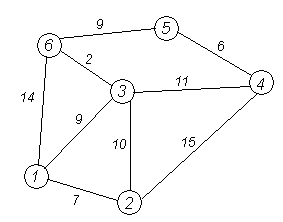
\includegraphics[width=0.4\textwidth]{Dijkstra/Dijkstra_graph0.png}
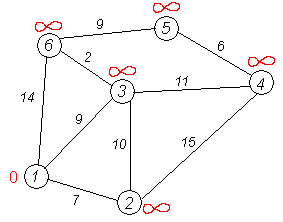
\includegraphics[width=0.4\textwidth]{Dijkstra/Dijkstra_graph1.png}

Пусть требуется найти кратчайшие расстояния от 1-й вершины до 5-й. Красным обозначим метки вершин, числами над рёбрами - веса. Можно условно понимать под весами расстояние между смежными вершинами.

Расставим метки: 1-ая вершина, так как является начальной, получит постоянную метку = 0, остальные вершины метку = \infty.

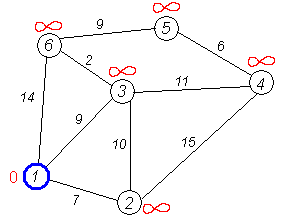
\includegraphics[width=0.4\textwidth]{Dijkstra/Dijkstra_graph2.png}
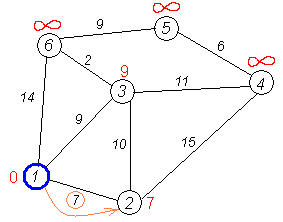
\includegraphics[width=0.4\textwidth]{Dijkstra/Dijkstra_graph3.png}

Начальная метка становится текущей (синий круг). Теперь выбираем из последующих вершин (2,3,6) одну. Возьмём вершину 2, потому что расстояние (вес) до неё минимально и равно 7. Пересчитаем её метку. Найдём сумму значения метки вершины 1 и длины ребра, идущего из 1-й в 2-ю, то есть 0 + 7 = 7. Это меньше текущей метки вершины 2, бесконечности, поэтому новая метка 2-й вершины равна 7.
Аналогичную операцию проделываем с двумя другими соседями 1-й вершины — 3-й и 6-й. Как только пересчитали все метки последующих вершин (2,3,6), превращаем наименьшую временную метку в постоянную метку, а вершину с этой меткой делаем текущей. Метка 2-ой вершины является наименьшей из всех временных.

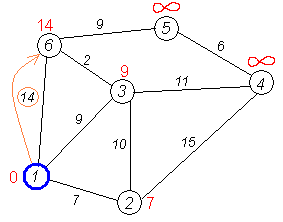
\includegraphics[width=0.4\textwidth]{Dijkstra/Dijkstra_graph5.png}
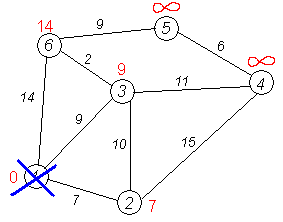
\includegraphics[width=0.4\textwidth]{Dijkstra/Dijkstra_graph6.png}

Пересчитываем метки последующих вершин для вершины 2. Метка 3-ей вершины = min(9,7*+10)=9, то есть не изменяется. Метка 4-ой вершины = min(\infty,7*+15)=22. Пересчитали все последующие временные метки. Теперь делаем метку 3-ей вершины постоянной, так как она имеет наименьшее значение. Последовательно повторим алгоритм для остальных вершин.

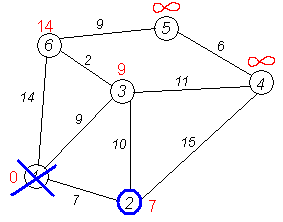
\includegraphics[width=0.4\textwidth]{Dijkstra/Dijkstra_graph7.png}
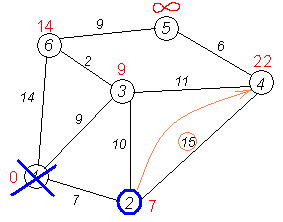
\includegraphics[width=0.4\textwidth]{Dijkstra/Dijkstra_graph8.png}

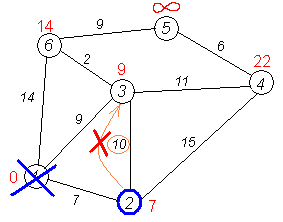
\includegraphics[width=0.4\textwidth]{Dijkstra/Dijkstra_graph9.png}
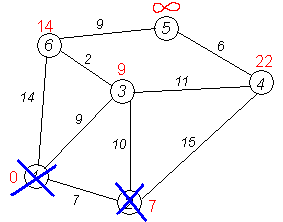
\includegraphics[width=0.4\textwidth]{Dijkstra/Dijkstra_graph10.png}

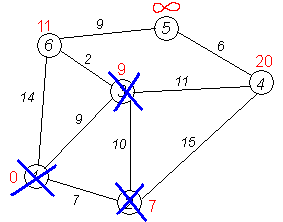
\includegraphics[width=0.4\textwidth]{Dijkstra/Dijkstra_graph11.png}
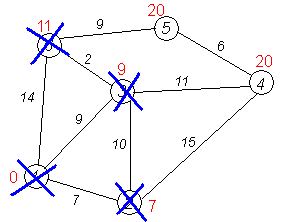
\includegraphics[width=0.4\textwidth]{Dijkstra/Dijkstra_graph12.png}

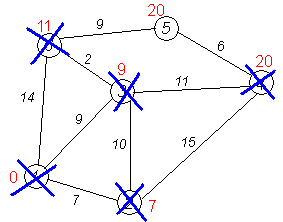
\includegraphics[width=0.4\textwidth]{Dijkstra/Dijkstra_graph13.png}
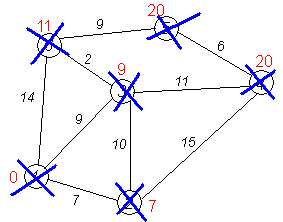
\includegraphics[width=0.4\textwidth]{Dijkstra/Dijkstra_graph14.png}

Теперь построим кратчайший путь. Для 5-ой вершины выбираем из 4-ой и 6-ой вершины такую, чтобы выполнялось равенство: метка 5-ой вершины = метка выбранной вершины + вес дуги от выбранной вершины до 5-ой. Видим, что 20 = 11 + 9 и 20 $\neq$ 20 + 6, поэтому выбираем 6-ую вершину. Делаем её текущей, а дугу (5,6) включаем в наш путь. Теперь этот же алгоритм повторяем для 6-ой вершины. Получим новую дугу (3,6). Затем для 3-ей вершины и получим (1,3).

Итак, кратчайший путь: (1,3) -> (3,6) -> (5,6)

\textbf{
Однако, чаще удобнее отмечать характеристики графа не на рисунке, а в матрице весов.
}

\subsection*{Пример из лекций Василия Павловича (с необходимым оформлением)}

Пусть дана матрица весов ориентированного графа. Необходимо найти кратчайший путь от $x_1$ до $x_6$.

\[
 \bordermatrix{ & x_1 & x_2 & x_3 & x_4 & x_5 & x_6 \cr
  x_1 & - & 5 & 10 & 13 & \infty & \infty  \cr
  x_2 & \infty & - & 8 & 9 & 13 & \infty  \cr
  x_3 & \infty & \infty & - & 5 & 3 & 6   \cr
  x_4 & \infty & \infty & \infty & - & 8 & 10  \cr
  x_5 & \infty & \infty & \infty & \infty & - & 9  \cr
  x_6 & \infty & \infty & \infty & \infty & \infty & - } \qquad
\] 

\textbf{1. Расстановка меток.}

Полагаем $d(x_1) = 0^*$ - постоянная метка, а
$d(x_2) = d(x_3) = d(x_4) = d(x_5) = d(x_6) = \infty$ - временные метки. Начальная метка становится текущей: $x_1 = \tilde x$.

\textbf{2. Изменение меток.}

Для всех вершин с временными метками, непосредственно следующими за $x_1$, пересчитываются метки по формуле. Заметим, что все они имеют вес, отличный от $\infty$ и --.
Множество этих вершин S =$\{ x_2, x_3, x_4 \}$.
\[ d_H(x_2) = min(d_C(x_2), d(\tilde x) + \omega(\tilde x, x_2 ) = min(d_C(x_2), d(x_1) + \omega(x_1, x_2 ) = min(\infty, 0^* + 5 ) = 5  \]
\[ d_H(x_3) = min(d_C(x_3), d(x_1) + \omega(x_1, x_3 ) = min(\infty, 0^* + 10 ) = 10  \]
Аналогично: $d_H(x_4) = 13$

\textbf{3. Превращение одной из временных меток в вершину с постоянной меткой }

\[ min\{d(x_2),d(x_3),d(x_4),d(x_5),d(x_6)\} = min\{5,10,13,\infty,\infty\} = 5 \]

Значит, вершина $x_2$ становится текущей $x_2 = \tilde x$, а её метка - постоянной $d(x_2) = 5^*$.

\textbf{4. Проверка окончания I этапа }

$x_2 = \tilde x \neq x_k \Rightarrow$ повторяем алгоритм, начиная со второго шага.

\textbf{2. Изменение меток.} 

S =$\{ x_3, x_4, x_5 \}. d_H(x_3) = min(10, 5^* + 8 ) = 10 $

$d_H(x_4) = min(13, 5^* + 9 ) = 13$

$d_H(x_5) = min(\infty, 5^* + 13 ) = 18$

\textbf{3. Превращение одной из временных меток в вершину с постоянной меткой }

\[ min\{d(x_3),d(x_4),d(x_5),d(x_6)\} = min\{10,13,18,\infty\} = 10 \]

Значит, вершина $x_3$ становится текущей $x_3 = \tilde x$, а её метка - постоянной $d(x_3) = 10^*$.

\textbf{4. Проверка окончания I этапа }

$x_3 = \tilde x \neq x_k \Rightarrow$ повторяем алгоритм, начиная со второго шага.

\textbf{2. Изменение меток.} 

S =$\{ x_4, x_5, x_6 \}. d_H(x_4) = 13, d_H(x_5) = 13, d_H(x_6) = 16$

\textbf{3. Превращение одной из временных меток в вершину с постоянной меткой: }
$min\{13,13,16\} = 13 \Rightarrow$ у вершин $x_4, x_5$ одинаковые метки $d(x_4)=d(x_5)=13$ можем выбрать одну из двух. Пусть $x_4 = \tilde x$, $d(x_4) = 13^*$

\textbf{4. Проверка окончания I этапа: } $x_4 = \tilde x \neq x_k \Rightarrow$ повторяем алгоритм, начиная со второго шага.

\textbf{2. Изменение меток.} S =$\{x_5, x_6 \}, d_H(x_5) = 13, d_H(x_6) = 16$

\textbf{3. Превращение одной из временных меток в вершину с постоянной меткой: } $min\{13,16\} = 13 \Rightarrow x_5 = \tilde x, d(x_5) = 13^*$

\textbf{4. Проверка окончания I этапа: } $x_5 = \tilde x \neq x_k \Rightarrow$ повторяем алгоритм, начиная со второго шага.

\textbf{2. Изменение меток.} S =$\{x_6 \},  d_H(x_6) = 16$

\textbf{3. Превращение одной из временных меток в вершину с постоянной меткой: } $x_6 = \tilde x$, $d(x_6) = 16^*$

\textbf{4. Проверка окончания I этапа: } $x_6 = \tilde x = x_k \Rightarrow$ начинаем II этап (построение пути), переходя к 5 шагу.

\textbf{5. Поиск дуг кратчайшего маршрута: }

$ x_k = x_6 = \tilde x = d(x_5) + \omega(x_5, \tilde x ) = 13 + 9 \Rightarrow 16 \neq 22 \Rightarrow x_5$ не подходит.

$\tilde x = d(x_4) + \omega(x_4, \tilde x ) \neq 23 \Rightarrow x_4$ не подходит.

$\tilde x = d(x_3) + \omega(x_3, \tilde x ) = 16 \Rightarrow x_3$ подходит. Включаем дугу $(x_3,x_6)$ в кратчайший путь. $x_3 = \tilde x$

\textbf{6. Проверка окончания II этапа: }

$\tilde x = x_3 \neq x_H = x_1 \Rightarrow$> возвращаемся к 5 пункту.

\textbf{5. Поиск дуг кратчайшего маршрута: } $\tilde x = d(x_1) + \omega(x_1, \tilde x ) = 10 \Rightarrow x_1$ подходит. Включаем дугу $(x_1,x_3)$ в кратчайший путь. $x_1 = \tilde x$

\textbf{6. Проверка окончания II этапа: } $\tilde x = x_1 = x_H \Rightarrow$ кратчайший путь построен: (1,3) -> (3,6)

\end{document}
